\documentclass[10pt]{book}
\usepackage[margin=2cm]{geometry}
\usepackage[font=small]{caption}
\geometry{a4paper}
\usepackage[utf8]{inputenc}
%\usepackage[T1]{fontenc}
\usepackage[parfill]{parskip}
\usepackage{graphicx}
\usepackage{amssymb}
\usepackage{epstopdf}
\usepackage{natbib}
\usepackage{gensymb}
\usepackage[overload]{textcase}
\usepackage{longtable}
\usepackage{datenumber}
\usepackage{calc}
\usepackage{datetime}

\usepackage[usenames,dvipsnames]{color}
\definecolor{snow}{gray}{0.98}

\usepackage{listings}
\lstset{
inputencoding=latin1,
basicstyle=\scriptsize\ttfamily\color{BrickRed}\bfseries,
frame=single,
backgroundcolor=\color{snow},
moredelim=[l][\color{black}]{|},
moredelim=[l][\color{black}]{:},
moredelim=[l][\color{Aquamarine}]{=key|},
moredelim=[l][\itshape\color{NavyBlue}]{\#},
}

\DeclareGraphicsRule{.tif}{png}{.png}{`convert #1 `dirname #1`/`basename #1 .tif`.png}

\usepackage[colorlinks=true, pdfstartview=FitV, linkcolor=blue,
            citecolor=blue, urlcolor=blue]{hyperref}

%\includeonly{Chapter1}

\renewcommand*{\familydefault}{\sfdefault}
\newdateformat{mydate}{\monthname[\THEMONTH] \THEYEAR}


% ------ local variables
\newcommand{\release}{2.6.4}
\newcommand{\releasename}{v\release}
\newcommand{\releasedate}{\mydate\today}
\newcommand{\webobs}{\textbf{WebObs }}
\newcommand{\wo}[1]{\MakeTextUppercase{#1}}
\newcommand{\wofile}[1]{\small{\textbf{#1}}}
\newcommand{\wokey}[1]{\fontfamily{lmtt}\fontseries{b}\selectfont\small#1\fontfamily{\sfdefault}\selectfont}
\newcommand{\wocmd}[1]{\textbf{#1}}

\newcounter{dateone}\newcounter{datetwo}
\newcommand{\yeartiltoday}[3]{
\setmydatenumber{dateone}{\the\year}{\the\month}{\the\day}
\setmydatenumber{datetwo}{#1}{#2}{#3}
\addtocounter{dateone}{-\thedatetwo}
\setcounter{dateone}{(\value{dateone}*100/36525)}\thedateone
}

\newtheorem{theorem}{Theorem}
\newtheorem{corollary}[theorem]{Corollary}
\newtheorem{definition}{Definition}
\newtheorem{lemma}{Lemma}
\newtheorem{exercise}{Exercise}
\newtheorem{remark}{Remark}
\newtheorem{example}{Example}
\newtheorem{warning}{Warning}

\def\grad{ \mbox{grad}}
\def\curl{ \mbox{curl}}
\def\div{ \mbox{div}}
\def\U{\ensuremath {\cal U}}
\def\S{\ensuremath {\cal S}}
\def\V{\ensuremath {\cal V}}
\def\R{\ensuremath {\cal R}}
\def\tr{\ensuremath {\mbox{tr}}}



% ------------------- Title and Author -----------------------------
\title{
	\includegraphics[height=5cm]{figures/logo_WebObs_C413.png}\\[1cm]
	%\includegraphics[height=3cm]{figures/LogoIPGP_petit.png}\quad
	%\includegraphics[height=2.5cm]{figures/LogoPRES.png}\quad
	%\includegraphics[height=2.5cm]{figures/logo_p7.png}\quad
	%\includegraphics[height=2.5cm]{figures/CNRSfilaire-grand.jpg}
	%\\[3cm]
	{\Huge \textbf{WebObs: An integrated web-based system for networks management and data monitoring in observatories}\\[.5cm]
\huge User and Administration Manual}\\[3cm]
	
\includegraphics[height=3cm]{figures/ipgp_up_verticaux_rvb.png}
}
\author{\textit{François Beauducel, Didier Lafon and Lucas Dassin}\\Institut de Physique du Globe de Paris Observatories\\}
\date{Release \releasename, \releasedate}


\begin{document}

% ==================================================================
\frontmatter

\maketitle
\tableofcontents
%%%%%%%%%%%%%%%%%%%%%%%%%%%%%%%%%%%%%%%%%%%%%%%%%%%%%%%%%%%%%%%%%%%%
%%%%%%%%%%%%%%%%%%%%%%%%%%%%%%%%%%%%%%%%%%%%%%%%%%%%%%%%%%%%%%%%%%%%

\chapter{Introduction}

\webobs is an integrated web-based system for data monitoring and networks management. Seismological and volcanological observatories have common needs and often common practical problems for multi disciplinary data monitoring applications. In fact, access to integrated data in real-time and estimation of uncertainties are keys for an efficient interpretation, but instruments variety, heterogeneity of data sampling and acquisition systems lead to difficulties that may hinder crisis management. In the Guadeloupe observatory, we have developed in the last 15 years an operational system that attempts to answer the questions in the context of a pluri-instrumental observatory. Based on a single computer server, open source scripts (with few binaries) and a Web interface, the system proposes:

\begin{itemize}
	\item  an extended database for networks management, stations and sensors (maps, station file with log history, technical characteristics, meta-data, photos and associated documents);
	\item  a web-form interfaces for manual data input/editing and export (like geochemical analysis, some of the deformation measurements, …); routine data processing with dedicated automatic scripts for each technique, production of validated data outputs, static graphs on preset moving time intervals, possible e-mail alarms, sensors and station status based on data validity;
	\item  in the special case of seismology, a multichannel continuous stripchart associated with EarthWorm~\footnote{see \url{http://www.isti.com/products/earthworm/}} and SeisComP3~\footnote{see \url{http://www.seiscomp3.org/}} acquisition chain, event classification database, automatic shakemap reports, regional catalog with associated hypocenter maps.
\end{itemize}

\webobs is presently fully functional and used in a dozen observatories, but the documentation is mostly incomplete. We hope to shortly finish the main user’s manual. If you are in a hurry, please contact the project coordinator and we will be happy to help you to install it. \webobs is fully described in the following paper: please cite this one if you publish something using \webobs:

\fbox{\parbox{\textwidth}{\small Beauducel F., D. Lafon, X. Béguin, J.-M. Saurel, A. Bosson, D. Mallarino, P. Boissier, C. Brunet, A. Lemarchand, C. Anténor-Habazac, A. Nercessian, A. A. Fahmi (2020). WebObs: The volcano observatories missing link between research and real-time monitoring, \textit{Frontiers in Earth Sciences}, \textbf{8}(47), \url{https://doi:10.3389/feart.2020.00048}.}}

% ==================================================================
\mainmatter

%%%%%%%%%%%%%%%%%%%%%%%%%%%%%%%%%%%%%%%%%%%%%%%%%%%%%%%%%%%%%%%%%%%%
%%%%%%%%%%%%%%%%%%%%%%%%%%%%%%%%%%%%%%%%%%%%%%%%%%%%%%%%%%%%%%%%%%%%
\definecolor{charcoal}{gray}{0.30}
\lstdefinestyle{console}
{language=bash,
basicstyle=\scriptsize\ttfamily\color{white}\bfseries,
backgroundcolor=\color{charcoal},
keywordstyle=\color{white},
alsoletter={:~\$},
}

\chapter{Installation}

% ==================================================================
\section{Overview}

\begin{figure}[!h]
	\centering
	\includegraphics[width=\textwidth]{figures/bigwo.pdf}
	\caption{\webobs big picture}
\end{figure}

% ==================================================================
\section{System requirements}

\subsection{System and package}

\webobs server can run on most \textbf{Linux} systems.

It has been successfully installed/tested on:
\begin{itemize}
\item   Linux 3.13.0 , x86\_64 , Ubuntu 14.04 LTS
\item   Linux 4.13.0 , x86\_64 , Ubuntu 16.04 LTS
\item   Linux 4.15.0 , x86\_64 , Ubuntu 18.04 LTS
\item   Linux 2.6.32, i386 , Debian 2.6.32-48squeeze4
\item   Linux version 3.2.0-4-amd64, Debian 3.2.51-1
\item   Linux version 3.2.0-4-amd64, Debian 4.6.3-14
\item   Linux version 4.9.0-5-amd64, Debian 4.9.65-3
%\item   Mac OS X 10.11.5, Darwin 15.5.0
\end{itemize}

\webobs (browser) clients have been successfully tested with:
\begin{itemize}
\item   FireFox (up to FireFox 93)
\item   Safari (up to Safari 14)
\end{itemize}

\fbox{
	\parbox{\textwidth}{
	Download  the \webobs latest Release and \textbf{MatLab} Runtime Compiler from:\\
	\url{https://ipgp.github.io/webobs/}
	}
}

% -----------------------------------------------------------------
\subsection{Software requirements}

\subsubsection{Required installations}

The following softwares will be tested for existence by the \textbf{setup} installation procedure:

\begin{itemize}
\item   Perl 5.14+ (\textbf{setup} will also check for additional Perl modules)
\item   Apache 2.2+
\item   Sqlite 3.7.9
\item   ImageMagick 6.6.9 (convert+identify)
\item   Mutt 1.5+
\item   MatLab MCR R2011b
\end{itemize}

\subsubsection{Bundled software}

The following lists softwares included in \webobs package:

\begin{itemize}
\item   SeisComP3 (slinktool + arclink\_fetch)
\item   JavaScript extensions:
\begin{itemize}
\item   JQuery
\item   flot
\item   markItUp
\item	MultiMarkDown
\item   overlib
\end{itemize}
\end{itemize}

% ==================================================================
\section{Initial installation}

You must have \textbf{root} privileges to execute \webobs installation. 

\textbf{Installation procedure}:

\begin{itemize}
\item   Choose/create your target \webobs directory, and \wocmd{cd} to it. For
demonstration purposes in this document we will use \wocmd{/opt/webobs/} as the target \webobs directory. 
\item   Download \webobs package and \textbf{MatLab RunTime Compiler}. For
demonstration purposes in this document we will use \wocmd{WebObs-\release.tgz} as the \webobs package. 
\item   Choose/create the system's \webobs user+group (aka \wocmd{WebObs Owner}) if you don't want \wocmd{setup} procedure
to create one itself.

\fbox{
	\parbox{\textwidth}{
	The \webobs \textbf{user}, and its corresponding \textbf{group}, is the required \webobs administration account. 
	It must have a home directory. It will be the owner of the \webobs CONF,LOGS,DATA,WWW,OUTx directories.  
	The Apache http server user will be made a member of \webobs user's group.
	The \webobs user can be used to launch the \webobs Scheduler and Postboard daemons.
	}
}

\item   Untar \webobs package. This will create/populate the \webobs version subdirectory: 
\wocmd{/opt/webobs/WebObs-\release}.
\item   Run the \wocmd{setup} procedure (again, with \wocmd{root} privileges):
\begin{itemize}
\item   must be called as \wocmd{/opt/webobs/WebObs-\release/SETUP/setup} (run \wocmd{setup -h} to see available options)
\item   \wocmd{setup} will gather information/location from your system/environment,
check for some dependencies (see Requirements section above), build the \webobs
structure, optionaly customize Apache's \webobs Virtual Host, set required system's
ownerships and access rights, install systemd services to manage the Postboard
and the Scheduler (on platforms using systemd), and populate your brand new
\webobs with ready-to-use demonstration data and templates.
\item   once completed, \wocmd{setup} will display \webobs configuration (see \wocmd{qsys} command below).
\item   \webobs now ready, you need to activate the \wocmd{scheduler}, \wocmd{postboard} and (re)start Apache http server. 
\end{itemize}
\end{itemize}

\begin{figure}[!h]
	\centering
	\includegraphics[width=\textwidth]{figures/disk_overview.pdf}
	\caption{Overview of \webobs installed disk structure}
\end{figure}

% ==================================================================
\section{Upgrades}

You must have \textbf{root} privileges to execute \webobs upgrades.

The \wocmd{setup} procedure used for Initial Installation, is also used to upgrade \webobs to a new release.
It will automatically detect that an upgrade is intended rather than a first time installation.

\textbf{Upgrade procedure:}

\begin{itemize}
\item   Download \webobs package corresponding to the version you want to upgrade to.
\item   Untar \webobs package.
\item   Run the \wocmd{setup} procedure by running the script \wocmd{/opt/webobs/WebObs-\release/SETUP/setup} (use the \wocmd{-h} option to see the help screen).
\item   \wocmd{setup} reports Version changes and important information in the
\wocmd{SETUP.CONF.README} file. Please read it carefully.
\item   if you choose to do so, \wocmd{setup} will also append to the
	configuration files of your installation (WebObs, Scheduler, and Grids
	configuration files, etc.) the configuration variables introduced by the
	current release and let you edit all the updated files to review or adapt
	the changes.
\end{itemize}

% ==================================================================
\section{qsys - query configuration}

\wocmd{qsys} script, also automatically executed when \wocmd{setup} ends, will
display your base \webobs configuration.

\begin{lstlisting}[style=console,title=\wofile{qsys} example]
                                     __ __ __
             ...oooooWoooooo..     W \ V  V /          Id: ipgp
          .oo.. ............o..o.. W  \_/\_/      Version: WebObs-2.0.0
       .oo.     ..............  ..oW   ___ 
     .oo.      ...............     W  / -_)         Owner: webobs[webobs]
    .W..     .  .............o.... W  \___|          Root: /opt/webobs
   .W.............o.........oWWWoo.W   _           Config: /opt/webobs/CONF/WEBOBS.rc
  .W    .   .  . ............o.....W  | |__          Logs: /opt/webobs/LOGS
  W.        ..   .WWWWo....  .     W  | '_ \
 .W        .Wo. .Wxxxxx....        W  |_.__/          MCR: /usr/local/MATLAB/MATLAB_Compiler_Runtime/v7...
 .W        .WWW.WxxxxxxW...   ...  W   ___        Rawdata: /opt/rawdata
 .W       .WWWWWxxxxxxxxW..........W  / _ \        Sefran: /opt/sefran
  Wo..ooWxxxxxxWxxxxxxxxxxo........W  \___/
  .xxxxxxxxxxxxxxWxxxxxxxxxW.......W   _             HTTP: http://webobs.ipgp
   .xxxxxxxxxxxxxWWWWWxxxxxxW.....oW  | |__                /etc/apache2/sites-available/webobs
    .WxxxxxxxxxWxxWWWWWWWxxxxxWWo..W  | '_ \               running on Apache/2.2.22 (Ubuntu)
     .oxxxxxxxxxxxxxWWWWWWWxxxxxxxWW  |_.__/
       .oWxxxxxxxxxxxxxWWWWWWWWxxxWW   ___      Scheduler: not running
          .oWxxxxxxxxxxxxWWWWWxW.. W  (_-<      PostBoard: not running
             ...oWWWxxxWWWWo..     W  /__/
                                                                qsys run 2014-08-08 12:05:06

\end{lstlisting}

% ==================================================================
\section{Configuration files syntax}

\webobs configuration files (*.rc, *.conf, or *.cnf) used to customize your installation
and described in this document, typically define one 
functionnal parameter (\wocmd{key}) per line, made up of one or more associated values
(\wocmd{fields}). They can share the same set set of syntactic rules for  
parsing/interpretation:

1) In order to be parsed/interpreted according to the following rules, the files must
contain a so-called 'definition line' (identified with \wocmd{=} in column 1) as the 
first interpreted line. This definition line is also used to further define parsing, 
that comes in two (2) flavors:

\begin{tabular}{ll}
\wocmd{=key\textbar value}  &  one value per key (Perl's equiv. \$X\{key\} =\textgreater value)\\
\wocmd{=key\textbar name1\textbar ...\textbar nameN}  & multiple named values per key (Perl's equiv. \$X\{key\}\{name1\} =\textgreater value)\\
\end{tabular}

2) Any text following a \wocmd{\#} is considered a comment and discarded.

3) Blank lines are discarded, leading and trailing blanks too.

4) Fields separator character, within interpreted lines, is \textbar (pipe).

5) \wocmd{\textbar} and \wocmd{\#} characters that must belong to a field value may be 
'escaped' (ie. not interpreted as separator or comment respectively) by prefixing them 
with a \textbackslash .

6) Field value substitution (interpolation) is allowed in \wocmd{=key\textbar value} format:

\begin{tabular}{ll}
\wocmd{\$\{key\} in value}       & will be replaced with the value of the key \textbar value pair of the current file.\\
\wocmd{\$WEBOBS\{key\} in value} & will be replaced with the value of the \webobs main configuration \wocmd{key} value. \\
\end{tabular}


% ==================================================================
\section{\webobs tree}
%\begin{table}[p]
\begin{center}
    \begin{longtable}{ll}
		\fcolorbox[gray]{0.1}{0.9}{\wocmd{CONF/}} & configurations  \\
	    \hspace{0.4cm} \wocmd{WEBOBS.rc}             & main \webobs configuration file  \\
	    \hspace{0.4cm} \wocmd{*.\{rc,conf,cnf\}}     & other configuration files \\
	    \hspace{0.4cm} \wocmd{FORMS/}                & FORMS definitions \\
	    \hspace{0.8cm} \wocmd{formname/}             & definitions for FORM formname    \\
	    \hspace{0.4cm} \wocmd{PROCS/}                & PROCS definitions \\
	    \hspace{0.8cm} \wocmd{procname/}             & definitions for PROC procname    \\
	    \hspace{0.4cm} \wocmd{SEFRANS/}              & SEFRANS definitions \\
	    \hspace{0.8cm} \wocmd{sefranname/}           & definitions for SEFRAN sefranname    \\
	    \hspace{0.4cm} \wocmd{VIEWS/}                & VIEWS definitions \\
	    \hspace{0.8cm} \wocmd{viewname/}             & definitions for VIEW viewname    \\
	    \hspace{0.4cm} \wocmd{GRIDS2FORMS/}          & links from PROCs to FORMS  \\
	    \hspace{0.8cm} \wocmd{PROC.pname.formname}   & -\textgreater ../formname  \\
	    \hspace{0.4cm} \wocmd{GRIDS2NODES/}          & links from GRIDs to NODES  \\
	    \hspace{0.8cm} \wocmd{PROC.pname.nodename}   & -\textgreater ../../DATA/NODES/nodename  \\
	    \hspace{0.8cm} \wocmd{VIEW.vname.nodename}   & -\textgreater ../../DATA/NODES/nodename  \\
	    \hspace{0.4cm} \wocmd{MENUS/}                & group's menus \\
	    \hspace{0.8cm} \wocmd{+GID}                  & menu content for group +GID \\
	    \\
		\fcolorbox[gray]{0.1}{0.9}{\wocmd{CODE/}} & \webobs code  \\
	    \hspace{0.4cm} \wocmd{bin/}                  & executables                \\
	    \hspace{0.4cm} \wocmd{cgi-bin/}              & Perl CGIs                  \\
	    \hspace{0.4cm} \wocmd{css/}                  & HTML Style Sheets          \\
	    \hspace{0.4cm} \wocmd{html/}                 & static HTML pages          \\
	    \hspace{0.4cm} \wocmd{icons/}                & HTML icons, static images  \\
	    \hspace{0.4cm} \wocmd{js/}                   & javascript                 \\
	    \hspace{0.4cm} \wocmd{matlab/}               & Matlab codes and library   \\
	    \hspace{0.4cm} \wocmd{python/}               & Python codes and library   \\
	    \hspace{0.4cm} \wocmd{shells/}               & bash commands              \\
	    \hspace{0.4cm} \wocmd{tplates/}              & configurations templates   \\
	    \\
		\fcolorbox[gray]{0.1}{0.9}{\wocmd{DATA/}} & data \\
	    \hspace{0.4cm} \wocmd{DB/}                  & built-in tools data         \\
	    \hspace{0.8cm} \wocmd{*.DAT}                & \\
	    \hspace{0.4cm} \wocmd{DEM/}                 & Digital Elevation Model files \\
	    \hspace{0.4cm} \wocmd{NODES/}               & NODES configurations and data \\
		\hspace{0.8cm} \wocmd{nodename/}            & nodename \\
		\hspace{1.2cm} \wocmd{*.txt}                & system features descriptions \\
		\hspace{1.2cm} \wocmd{*.cnf}                & configuration                \\
		\hspace{1.2cm} \wocmd{*.clb}                & calibration file             \\
		\hspace{1.2cm} \wocmd{DOCUMENTS/}           & documents                    \\
		\hspace{1.2cm} \wocmd{FEATURES/}            & features                     \\
		\hspace{1.2cm} \wocmd{EVENTS/}              & events log                   \\
		\hspace{1.2cm} \wocmd{PHOTOS/}              & pictures                     \\
	    \\
		\fcolorbox[gray]{0.1}{0.9}{\wocmd{DOC/}} & documentations  \\
	    \\
		\fcolorbox[gray]{0.1}{0.9}{\wocmd{LOGS/}} & tools, appl, daemons logs  \\
	    \\
		\fcolorbox[gray]{0.1}{0.9}{\wocmd{OUTG/}} & batch Procs Outputs  \\
		\hspace{0.4cm} \wocmd{PROC.procname/}       & PROC procname outputs \\
		\hspace{0.8cm} \wocmd{exports/}             &  \\
		\hspace{0.8cm} \wocmd{graphs/}              &  \\
		\hspace{0.8cm} \wocmd{maps/}                &  \\
		\hspace{0.8cm} \wocmd{events/}              &  \\
	    \\
		\fcolorbox[gray]{0.1}{0.9}{\wocmd{OUTR/}} & Procs Requests Outputs  \\
		\hspace{0.4cm} \wocmd{20140720\_084340\_85.199.99.199\_userX/}    & Dated Request  \\
		\hspace{0.8cm} \wocmd{REQUEST.rc}          &  Request parameters \\
		\hspace{0.8cm} \wocmd{PROC.procname/}      &  Requested Proc outputs \\
		\hspace{1.2cm} \wocmd{graphs/}             &   \\
		\hline
    \end{longtable}
\end{center}
%\end{table}


% ==================================================================
\section{License}


%%%%%%%%%%%%%%%%%%%%%%%%%%%%%%%%%%%%%%%%%%%%%%%%%%%%%%%%%%%%%%%%%%%%
%%%%%%%%%%%%%%%%%%%%%%%%%%%%%%%%%%%%%%%%%%%%%%%%%%%%%%%%%%%%%%%%%%%%
\chapter{Reference}

% ==================================================================
\section{Overview}

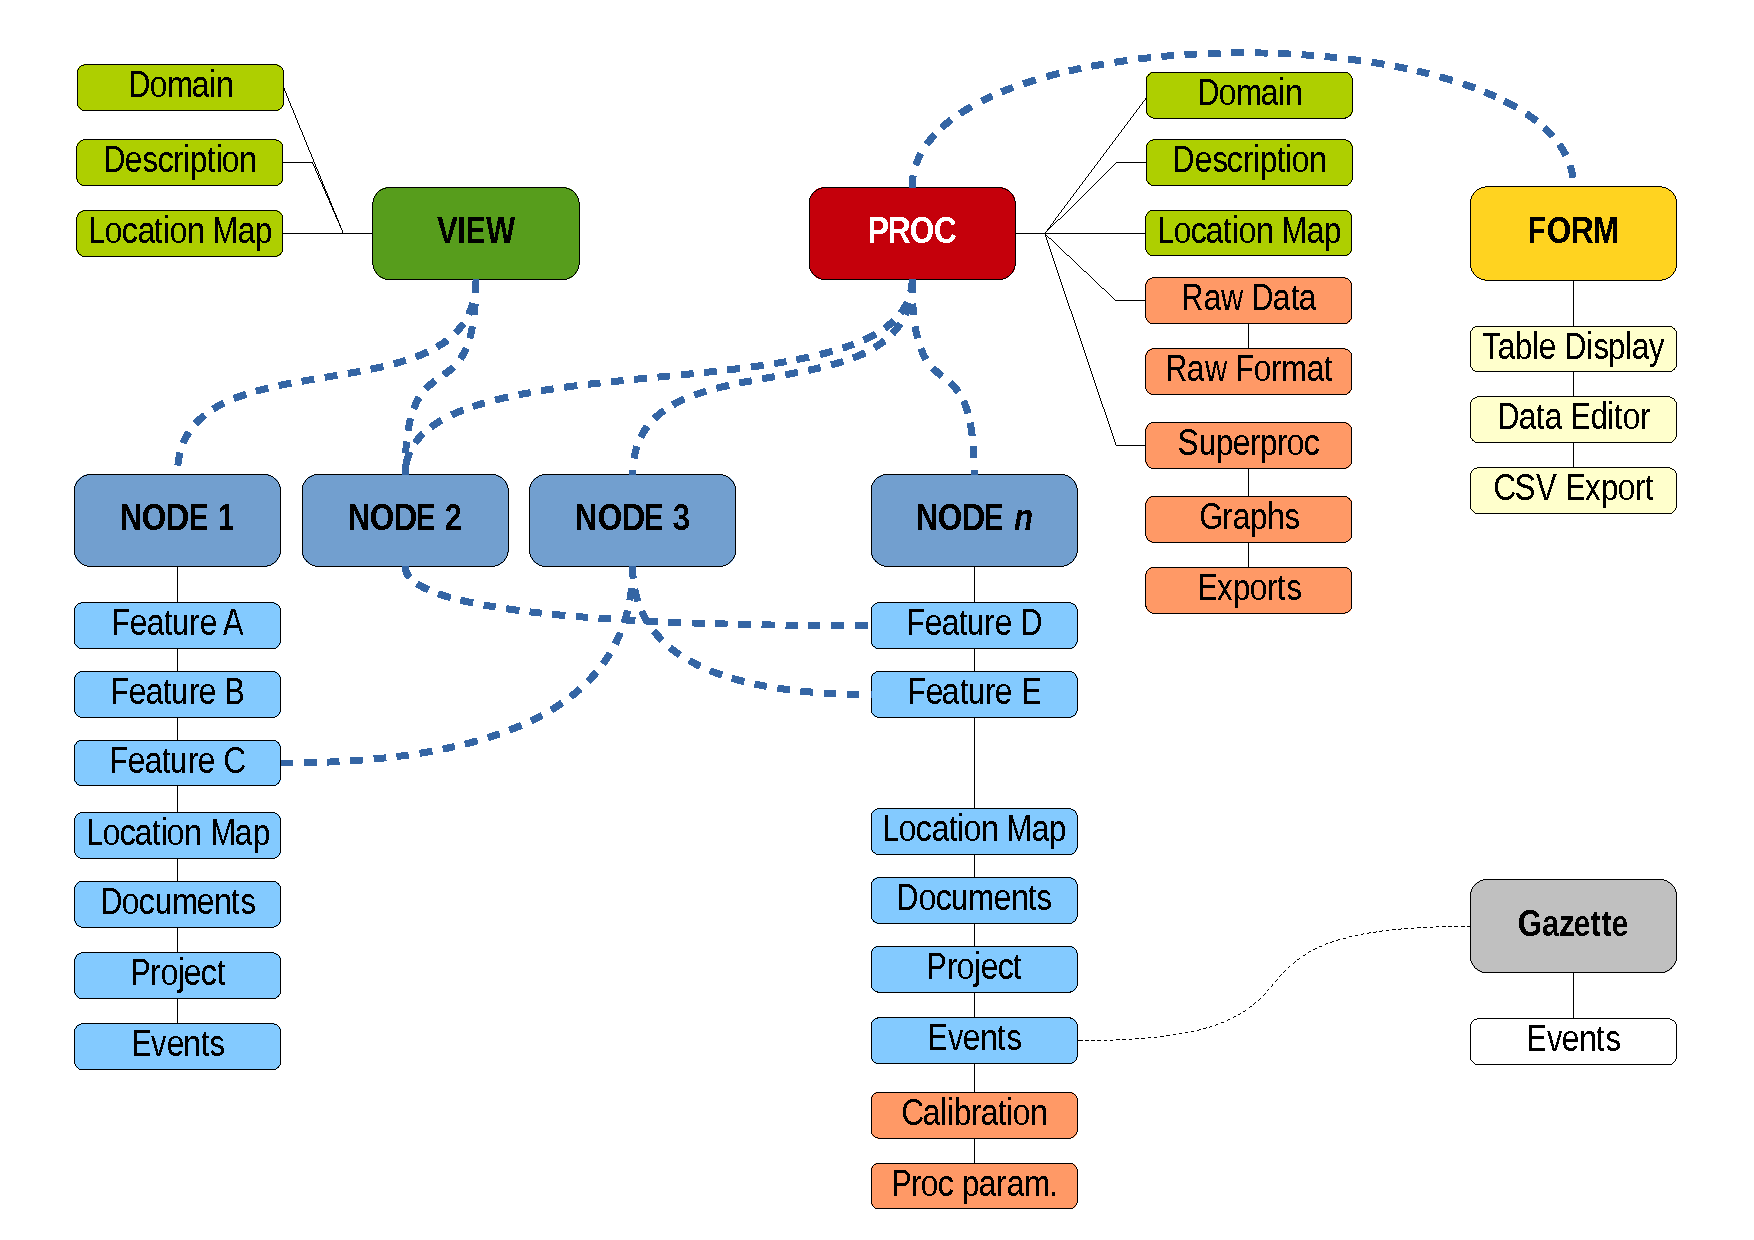
\includegraphics[width=\textwidth]{figures/webobs_diagram.pdf}

% ==================================================================
\section{Nodes: Elementary WebObs Objects}

A \wo{node} is the central \webobs element associated with following attributes:

\begin{itemize}
\item    a long name (\wo{name}) and short name (\wo{alias});
\item    an optional short description (\wo{type});
\item    a lifetime period with start and end dates (both optional);
\item    an optional location (latitude, longitude, elevation) associated with a location map (graph), Google Maps and Google Earth links;
\item    optional text contents for "informations", "installation" and "access";
\item    an optional sensor description associated with a calibration table of channels parameters;
\item    a list of user-defined features (also free text contents);
\item    attached documents, photos and diagrams;
\item    a project;
\item    events log associated with date and operator list;
\item    a list of associated grids (\wo{views} and/or \wo{procs}, see \ref{grids});
\item    a validity flag (for admin users);
\item	 optional functional parameters when the \wo{node} is associated to a \wo{proc}: data code (\wo{FID}), network code (\wo{FDSN}), data format (\wo{RAWFORMAT}) and source (\wo{RAWDATA}), time zone (\wo{TZ}), acquisition period and delay, and a calibration file that describes each channel characteristics and history:
	\begin{itemize}
	\item    date and time of validity;
	\item    channel number, name, unit, code, S/N, offset, factor, gain, min/max values, azimuth, latitude, longitude, elevation, depth, sampling frequency, dynamic, location code.
	\end{itemize}
\end{itemize}

Examples of what a \wo{node} can be:
\begin{itemize}
\item    an instrumental station or a part of it,
\item    a site or place for data sampling or measurement,
\item    a place of any interest,
\item    a mobile equipment, an instrument, a building, a vehicle, ...
\item    a journal board, an event description (e.g. an historical earthquake), ...
\end{itemize}


\lstinputlisting[title=\wofile{NODES.rc}]{../../SETUP/CONF/NODES.rc}

% -----------------------------------------------------------------
\subsection{Create, edit or delete a NODE}

Modifying \wo{node} is possible only through a \wo{grid} (see next section \ref{grids}). Creation of new \wo{node} or edition of an existing \wo{node} deserves to \wo{users} with edit level for the associated \wo{grid}. Deletion of a \wo{node} is reserved to administrator level \wo{users}.


% -----------------------------------------------------------------
\subsection{Names and codes}

% - - - - - - - - - - - - - - - - - - - - - - - - - - - - - - - - -
\subsubsection{Main code (ID)}

Each \wo{node} has a unique ID code in \webobs. The code can be any string of characters, but it is recommended to use a comprehensive and rational code (see appendix \ref{nodeidcodes}) when creating a new \wo{node}. Attribution of this unique code deserves to \wo{users} with administrator level when creating a new \wo{node}. It cannot be modified after.

% - - - - - - - - - - - - - - - - - - - - - - - - - - - - - - - - -
\subsubsection{Name}

The long NAME of a \wo{node} is used for display purposes in tables and graphs. It cannot be empty. The NAME is displayed in the main GRID's table in front of the corresponding \wo{node}.


% - - - - - - - - - - - - - - - - - - - - - - - - - - - - - - - - -
\subsubsection{Alias (short name)}

The ALIAS is the short name of a \wo{node}, used for display purposes in table and graphs. It cannot be empty. The ALIAS is displayed in the main GRID's table in front of the corresponding \wo{node}.



% - - - - - - - - - - - - - - - - - - - - - - - - - - - - - - - - -
\subsubsection{Type}

The TYPE of a \wo{node} is an optional free string that will be used for any short description of the \wo{node}. The TYPE is displayed in the main GRID's table in front of the corresponding \wo{node}.


% -----------------------------------------------------------------
\subsection{Lifetime and validity}

% - - - - - - - - - - - - - - - - - - - - - - - - - - - - - - - - -
\subsubsection{Start/end dates}

Start and end dates of a \wo{node} define the period of activity of this \wo{node}. Both or any of these two dates can be undefined or incompletely defined, while respecting the ISO 8601 standard: Date values are ordered from the most to the least significant: year, month and day; any number of values may be dropped from any of the date representations, but in the order from the least to the most significant. For example, 1976 and 2005-04 are both reduced precision valid dates.

The lifetime of a \wo{node} has potential impact on processes that use this \wo{node} or associated data.


% - - - - - - - - - - - - - - - - - - - - - - - - - - - - - - - - -
\subsubsection{Valid \wo{node}}

Independently of the lifetime period, a \wo{node} can be valid or invalid. When invalid, a \wo{node} is simply ignored by most of the \webobs processes and invisible for standard \wo{users}. Nevertheless, if a \wo{user} has an administrator level , he will be able to see an invalid \wo{node} in the lists and tables.



% -----------------------------------------------------------------
\subsection{Grids memberships}

A \wo{node} can be associated with one or more \wo{grids}. See section \ref{grids}.

% -----------------------------------------------------------------
\subsection{Geographic location}

\includegraphics[width=\textwidth]{figures/NODE_location.png}

A \wo{node} can be georeferenced using latitude, longitude and elevation coordinates on Earth. When a \wo{node} has valid coordinates defined, a location map will be automatically built (see below and section \ref{locastat}), and it will appear on associated GRID's maps (see section \ref{grids}).

% - - - - - - - - - - - - - - - - - - - - - - - - - - - - - - - - -
\subsubsection{WGS84 coordinates}

Latitude and longitude must be in the WGS84 geodetic reference system, and expressed in decimal form, using negative value for southern latitude and western longitude. Use the dot as decimal point (not coma).

In the \wo{node}'s display page, coordinates are presented in different formats: DDD.ddddd (decimal degrees), DDD\degree MM.mmm' (degrees and decimal minutes) and DDD\degree MM'SS.s" (degrees, minutes and decimal secondes).

The coordinates are displayed in the main GRID's table in front of the corresponding \wo{node}. Also, the Universal Transverse Mercator (UTM) projection is computed and displayed in the \wo{node}'s page.

% - - - - - - - - - - - - - - - - - - - - - - - - - - - - - - - - -
\subsubsection{Timestamp and type of coordinates}

This optional information provides the timestamp (date) of coordinates, and a type of positioning from a list.

\lstinputlisting[title=\wofile{POSITIONtypes.conf}]{../../SETUP/CONF/POSITIONtypes.conf}


% - - - - - - - - - - - - - - - - - - - - - - - - - - - - - - - - -
\subsubsection{Google Maps API link}

Link to Google Maps API is available if the \wo{node} has coordinates. The link will open a pop-up window. This functionality is associated with some variables in the main configuration file \wofile{WEBOBS.rc}:

\begin{lstlisting}[title=\wofile{WEBOBS.rc} (excerpt)]
CGI_GOOGLE_MAPS|googleMAPS.pl
GOOGLE_MAPS_LINK|1
GOOGLE_MAPS_API|http://maps.google.com/maps?file=api
GOOGLE_MAPS_API_KEY
GOOGLE_MAPS_LINK_INFO|See with Google Maps (ATTENTION: error ~20 m)
GOOGLE_MAPS_ICON|/icons/gdot.png
GOOGLE_MAPS_TYPE|G_HYBRID_MAP
GOOGLE_MAPS_WIDTH_VALUE|500
GOOGLE_MAPS_HEIGHT_VALUE|500
GOOGLE_MAPS_ZOOM_VALUE|17
\end{lstlisting}

% - - - - - - - - - - - - - - - - - - - - - - - - - - - - - - - - -
\subsubsection{Google Earth KML link}

Link to Google Earth KML file is available if the \wo{node} has coordinates. The link will download a local KML file, which may be open with local application Google Earth (if installed). This functionality is associated with some variables in the main configuration file \wofile{WEBOBS.rc}:

\begin{lstlisting}[title=\wofile{WEBOBS.rc} (excerpt)]
GOOGLE_EARTH_LINK|1
GOOGLE_EARTH_LINK_INFO|KML file for Google Earth (ATTENTION: error ~20 m)
IMAGE_LOGO_GOOGLE_EARTH|/icons/google/google_earth.gif
\end{lstlisting}

% - - - - - - - - - - - - - - - - - - - - - - - - - - - - - - - - -
\subsubsection{Location map}

A location map with 4 different scales is automatically made and updated by LOCASTAT application (see section \ref{locastat} for associated parameters), using the coordinates of the \wo{node}.


% -----------------------------------------------------------------
\subsection{Transmission}

When a \wo{node} represents, for instance, an instrumental station with data transmission, the type of transmission can defined using a reference list (below) and other \wo{node}s can be defined as intermediate repeaters or final acquisition point.

The transmission chain is displayed with dynamic links to associated \wo{node}s. It appears also on the location map (see section \ref{locastat}) and the \wo{grid} maps (see section \ref{gridmaps}).

% - - - - - - - - - - - - - - - - - - - - - - - - - - - - - - - - -
\subsubsection{Type}

Type of transmission is defined in a list of transmission type associated with plot line style, width and color.

\lstinputlisting[title=\wofile{TRANStypes.conf}]{../../SETUP/CONF/TRANStypes.conf}


% - - - - - - - - - - - - - - - - - - - - - - - - - - - - - - - - -
\subsubsection{Acquisition and repeaters}

The transmission chain is described by defining a list of \wo{node}'s ID, from station to acquisition.


% -----------------------------------------------------------------
\subsection{Proc's parameters and data status}
\label{nodeprocparam}
When associated with a \wo{proc} (see section \ref{procs}), data from a \wo{node} is used to produce outputs. Several additional parameters must be defined for this.


% - - - - - - - - - - - - - - - - - - - - - - - - - - - - - - - - -
\subsubsection{Network code}

A \wo{node} can be associated with a standard network code, from the International Federation of Digital Seismograph Networks (FDSN)~\footnote{see \url{http://www.fdsn.org/}}. This is mostly the case for permanent seismological stations. This code is mandatory when using Arclink or Seedlink data requests (see sections \ref{seedlink} and \ref{arclink}).

The list of network codes is also described at IRIS~\footnote{see \url{http://www.iris.edu/ds/nodes/dmc/services/network-codes/}}.

The official FDSN codes list can be overwritten using a local configuration file \wofile{CONF/networkcodes.csv}.

% - - - - - - - - - - - - - - - - - - - - - - - - - - - - - - - - -
\subsubsection{Raw format}

A list of possible data format that overwrites, if selected, the \texttt{RAWFORMAT} parameter in the PROC/*.conf. This allows to associate different data format/source to the NODEs associated to a single PROC.


% - - - - - - - - - - - - - - - - - - - - - - - - - - - - - - - - -
\subsubsection{Raw data source}

A free text string that overwrites, if not blank, the \texttt{RAWDATA} parameter in the PROC/*.conf. This allows to associate different data format/source to the NODEs associated to a single PROC.


% - - - - - - - - - - - - - - - - - - - - - - - - - - - - - - - - -
\subsubsection{FID}

A FID code is a short string which may contain a functional code (or a coma-separated list of codes) that will be used by associated PROCs. For example, it can be the official station code for a seismic station or a GNSS receiver, while the data files will contain this code. It is generally set to the same string as the ALIAS.

Some \wo{procs} are able to deal with a coma-separated list, as gnss: this allows to define multiple codes pointing to different data, and associate them to a single station.

% - - - - - - - - - - - - - - - - - - - - - - - - - - - - - - - - -
\subsubsection{FID\_*}

Some raw formats may need additional codes or parameters to process data from the \wo{node}. It is possible to define specific parameters with the prefix \wo{FID\_}: they will be listed and editable below the main FID. Creation/edit of a \wo{FID\_SUBNAME} is reserved to \wo{users} with administrator level.


% - - - - - - - - - - - - - - - - - - - - - - - - - - - - - - - - -
\subsubsection{Time zone}

Time zone is the offset delay from UTC, expressed in hours. Examples: $+0$ is UTC, $-4$ is Lesser Antilles time.

% - - - - - - - - - - - - - - - - - - - - - - - - - - - - - - - - -
\subsubsection{Acquisition period}

Acquisition period defines the normal time interval between two data sample, expressed in days. Examples: \texttt{1/24} corresponds to 1 sample per hour, \texttt{1/86400} is 1 Hz sampling. This value might be used to compute average acquisition performance rating (see below).

% - - - - - - - - - - - - - - - - - - - - - - - - - - - - - - - - -
\subsubsection{Acquisition delay}

This value defines the maximum delay allowed between the last available data and the present time, expressed in days. This delay is used to determine the \wo{node}'s status (see below).

% - - - - - - - - - - - - - - - - - - - - - - - - - - - - - - - - -
\subsubsection{Status and link to data}

If the associated \wo{proc} is set to compute the \wo{node} status, the following information is displayed:
\begin{itemize}
\item last status check timestamp;
\item sampling rate performance (in \%): number of valid samples over the last time period, compared to theoretical acquisition period (see above);
\item status (in \%): existence of valid samples in the last time delay for all channels.
\end{itemize}

The status informations are displayed in the main GRID's table in front of the corresponding \wo{node}.

If the associated \wo{proc} produces output graphs, direct links to each outputs are available.


% - - - - - - - - - - - - - - - - - - - - - - - - - - - - - - - - -
\subsubsection{Channels parameters (calibration file)}
\label{clb}

\includegraphics[width=\textwidth]{figures/CLB_table.png}

For most of \wo{procs}, it is mandatory to define a list of data channels. This can be done through a ``calibration file'' that contains description and detailed parameters of the \wo{node}'s data channels: date and time of validity, name, unit, S/N, functional code, gain and multiplier factors, offset, min/max values, sensor azimuth, location and depth, sampling frequency, digital dynamic and ``location code'' (SEED standard). Each channel must have one or more series of parameters. 

The date and time of validity applies until real-time or next line of parameters for this channel number.

Each \wo{proc} might be associated to a selection of channels. Active channels appear in bold font, while inactive appear in gray.

% -----------------------------------------------------------------
\subsection{Features}

Each \wo{node} can have user-defined features which are free text contents (HTML and Wiki syntax allowed) that appear in the main table as a series of table cells.

% - - - - - - - - - - - - - - - - - - - - - - - - - - - - - - - - -
\subsubsection{List of user-defined features}

Feature name is limited to short names and must avoid special characters. Edit the list of features to be displayed using the \wo{node} configuration form. Features with void content won't be displayed for \wo{users} without edit or admin rights.

% - - - - - - - - - - - - - - - - - - - - - - - - - - - - - - - - -
\subsubsection{Node-features-nodes association list}

It is possible to associate a \wo{node}'s feature to an other \wo{node} as its feature's children. An automatic link will be displayed in the feature's table cell before the text content of the feature. In the children \wo{node} page, the parent feature will appear with automatic name "feature of" and a link to the parent \wo{node}.

Configuring the node2node association list is made by editing a configuration file containing a 3-field definition (pipe delimited):

\begin{lstlisting}[title=\wofile{nodes2nodes.rc} (excerpt)]
PARENT_NODEID|featurename|CHILDREN_NODEID
\end{lstlisting}


% -----------------------------------------------------------------
\subsection{Installation, information and access}

These 3 fields are free-length text content. Wiki syntax allowed.

% -----------------------------------------------------------------
\subsection{Photos, diagrams and associated documents}

Three different types of documents can be uploaded and associated to a \wo{node}:
\begin{itemize}
	\item Photos: any JPEG file that will be displayed as thumbnail with a link to full screen mode;
	\item Diagrams: any image or picture file (JPEG, GIF, PNG, PDF, ...) that will be displayed as thumbnail with a link to the full resolution image;
	\item Documents: any file (PDF, DOC, TXT, ...) that will be downloadable and sometimes displayed through the navigator.
\end{itemize}


% -----------------------------------------------------------------
\subsection{Project}
\label{projectnode}

A \wo{node} may have one (and only one) \wo{Project} description: a free-length text file, accepting MultiMarkDown syntax, a list of users and possible associated photos. Project is a special \wo{Event} without date.

% -----------------------------------------------------------------
\subsection{Events}
\label{eventnode}

A \wo{node} can be associated to dated events. A \wo{node} event has following characteristics:
\begin{itemize}
	\item start date and time;
	\item end date \& time;
	\item a title;
	\item a content of free-length text,
	\item author(s) from the list of \webobs users;
	\item selected feature (from the node's feature list);
	\item sensor/data outcome flag;
	\item notebook number (optional);
	\item notebook forward flag (optional);
	\item associated photos (image files).
\end{itemize}
An event can include one or more sub-events (children). Event files  accept the MultiMarkDown syntax. See \wo{Events logging} section (\ref{events_logging}) for a description of Nodes and Grids events coding.


% ==================================================================
\section{Grids: networks of nodes}
\label{grids}

A \wo{grid} is a group of \wo{nodes}. Each \wo{node} can be associated to one or multiple \wo{grids}. There is two kind of \wo{grids}:

\begin{itemize}
\item    A \wo{view} is a list of \wo{nodes} we simply want to group to be seen or accessed together,
\item    A \wo{proc} is a list of \wo{nodes} associated to a common data processing that produces outputs (graphs and/or elaborated data), and/or optional editable data FORMS.
\end{itemize}

\wo{grids} are presented through a sorted table allowing access to dedicated page for each \wo{grid} with:
\begin{itemize}
\item    domain: a category used to group similar \wo{grids};
\item    purpose (text content);
\item    specifications: operator owner, number of \wo{nodes}, type, optional external link;
\item    list of \wo{nodes}: a complete table with alias, names, location, start/end dates, type, project, status (for active \wo{proc}); ...
\item    an interactive location map (if at least one \wo{node} is georeferenced);
\item    informations (text content);
\item    references (text content);
\item    a graphical representation of \wo{nodes} links with associated \wo{grids}.
\end{itemize}

Text content sections are editable with Wiki syntax possibilities.

%\includegraphics[width=\textwidth]{figures/PROC_GEOSCOPE_map.png}


\lstinputlisting[title=\wofile{GRIDS.rc}]{../../SETUP/CONF/GRIDS.rc}

% -----------------------------------------------------------------
\subsection{Domains}
\label{domains}

A \wo{domain} is a generic category that is used to group \wo{grids} together: in the \wo{grid}'s table presentation and in most of the page links between \wo{grids} and \wo{nodes}. By default, \wo{domains} are defined as a list of standard scientific methods as used in volcanological observatories: Seismology, Deformations, Geochemistry, Imagery, ... but these categories can be changed to better fit the \webobs needs. For example, if the \webobs has to handle multiple targets (like volcanoes), you might want to make the \wo{domains} as a list of these targets.

Changes to \wo{domains} list can be done by administrator by editing the sqlite database. New domains can be easily added by inserting an entry into the \wokey{domains} table. To remove an existing \wo{domain}, you must remove any \wo{grid} associated to this \wo{domain} first (this can be done using the GUI of \wo{grid} configuration editor), then delete manually the entry in the database. 

\begin{lstlisting}[title=\wofile{WEBOBS.rc} (excerpt)]
SQL_DOMAINS|${ROOT_CONF}/WEBOBSDOMAINS.db
SQL_TABLE_DOMAINS|domains
SQL_TABLE_GRIDS|grids2domains
\end{lstlisting}



% -----------------------------------------------------------------
\subsection{Views}
\label{views}

A \wo{view} is a simple group of NODES.

To create a new \wo{view}, go to any \wo{GRID} table page (menu GRIDS, VIEWS or PROCS) and click on the edit icon in the Name header of table, enter an unique short name and click Edit. This will open the \wo{grid} configuration editor. The form allows to freely edit the parameters file (key/value pairs), to select the Domain and to associate/disassociate \wo{nodes}.

\lstinputlisting[title=\wofile{VIEW.DEFAULT} template]{../../CODE/tplates/VIEW.DEFAULT}

All the following parameters are valid for \wo{grids}, that is any \wo{view} or \wo{proc} (see the next section).

% - - - - - - - - - - - - - - - - - - - - - - - - - - - - - - - - -
\subsubsection{\wo{grid} name and attributes}
\begin{itemize}

\item \wokey{NAME}: Character string for the \wo{grid} long name. This name will appear in the \wo{grid} page and maps of \wo{nodes}.

\item \wokey{OWNCODE}: Character string for the \wo{grid}'s owner name. This name will be displayed in the \wo{grids} tables and \wo{grid} summary, if \wokey{SHOW\_OWNER} key is true in \wofile{GRIDS.rc}. For backward compatibility, the key might contains a short code with corresponding long names in \wofile{CONF/OWNERS.conf}.

%\lstinputlisting[title=\wofile{OWNERS.conf} template]{../../SETUP/CONF/OWNERS.conf}

\item \wokey{TYPE}: Character string giving a short attribute to the \wo{grid}, if \wokey{SHOW\_TYPE} key is true in \wofile{GRIDS.rc}.

\item \wokey{URL}: Optional URL related to the \wo{grid}. Any valid URL is allowed, e.g. an external web link.

\item \wokey{COPYRIGHT}: Optional character string for the copyright of the \wo{grid}.

\end{itemize}


% - - - - - - - - - - - - - - - - - - - - - - - - - - - - - - - - -
\subsubsection{\wo{NODES} attributes}
\begin{itemize}

\item \wokey{NODE\_NAME}: Short name of a generic \wo{node}. This name will be used instead of ``node'' in tables and maps.

\item \wokey{NODE\_MARKER}: Type of marker used to plot \wo{nodes} on maps. See valid markers in table \ref{markertype}.

\item \wokey{NODE\_SIZE}: Size of the \wo{node} marker for maps (in points).

\item \wokey{NODE\_RGB}: Color of the \wo{node} marker for maps: it can be a color name string (see \wofile{CODE/matlab/htm2rgb.m} for a list of standard colors), or a vector of 3 scalars (red,green,blue), each value between 0 and 1.

\item \wokey{NODE\_FONTSIZE}: If not empty, font size to display \wo{node}'s alias names on maps besides the marker.

\end{itemize}

% - - - - - - - - - - - - - - - - - - - - - - - - - - - - - - - - -
\subsubsection{Digital Elevation Model (DEM)}
\label{dem}

For any \wo{view} or \wo{proc} that needs topographic data, \webobs will use either SRTM3, SRTM1, ETOPO5, ETOPO1 or user-defined DEM file. SRTM tiles will be downloaded automatically from internet, as needed by the PROC, and stored in the \wokey{PATH\_DATA\_DEM} local directory (see \wofile{WEBOBS.rc}). ETOPO5 is available in the \webobs package offline. ETOPO1 must be downloaded manually from the web. The selection between these different sources respects the following policy:
\begin{enumerate}

\item SRTM3 is the default, 90m resolution worldwide DEM, available through $1\times1^o$ tiles. It is convenient for any maps from about 20km to 500km width. \wofile{WEBOBS.rc} defines a limit of \wokey{SRTM\_MAX\_TILES} as maximum amount of tiles to avoid memory issues (default is 25). If the covered area needs more than this limit, it will switch automatically to ETOPO with a warning in the logs.

\item SRTM1, a 30m resolution DEM can be activated setting \wokey{DEM\_SRTM1} to \wokey{Y} in the PROC's configuration file. Each tile is $1\times1^o$ and 9 times bigger than SRTM3. This is convenient for smaller areas less than 20km width. \wofile{WEBOBS.rc} defines a limit of \wokey{SRTM1\_MAX\_TILES} maximum amount of tiles to avoid memory issues (default is 4). If the covered area needs more than this limit, it will switch automatically to SRTM3 with a warning in the logs.

\item if SRTM3 or SRTM1 limits are exceeded for any large area, \webobs will use ETOPO worldwide DEM with bathymetry. ETOPO5 is 5 arc-min resolution (about 9km) which is convenient for maps greater than 2,000km width. If ETOPO1 has been installed (which is recommended at installation), it offers 1 arc-min resolution (about 1.8km) which is convenient for maps width greater than 500km. So with SRTM and ETOPO1 installed, most situations will produce nice basemaps.

\item if the area is less than about 5km width, even SRTM1 is not enough to produce decent maps. In that case it is more appropriate to use a local DEM file (in ArcInfo ascii format, elevation values in meters) that can be defined in the PROC's configuration file with \wokey{DEM\_FILE} as full path of the file, and \wokey{DEM\_TYPE} as \wokey{LATLON} (preferred) or \wokey{UTM} (might takes more time). If this DEM does not cover the whole area, the PROC will switch automatically to SRTM/ETOPO data. Nevertheless, it is possible to force the use of your local DEM by setting \wokey{DEM\_FORCED} to \wokey{Y} but when the area exceeds the DEM data, map will be surrounded by gray zones where there is no data available. A last option \wokey{DEM\_COPYRIGHT} allows to specify the DEM copyright.

\end{enumerate}



% -----------------------------------------------------------------
\subsection{Procs}
\label{procs}

A \wo{proc} is a list of \wo{nodes} that are associated to a specific and common data processing called \wo{superproc}. It has the same basic parameters as \wo{views} (see previous section \ref{views}) plus additional settings that depend on the process you want to achieve. \webobs proposes some built-in \wo{superprocs} (see chapter \ref{builtin}), each of them are specific. There is on default \wo{superproc} called 'genplot' which is a simple plot of time series data (see section \ref{genplot}).

To create a new \wo{proc}, go to any \wo{GRID} table page (menu GRIDS, VIEWS or PROCS) and click on the edit icon in the Name header of table, select ``PROC: Generic time series'' in the Grid type list, enter an unique short name and click Edit. This will open the \wo{proc} configuration editor. The form allows to freely edit the parameters file (key/value pairs), to select the Domain, optional \wo{form} and to associate/disassociate \wo{nodes}.

\label{forms}

A \wo{form} is a web interface for manual data input, edit, display and export. A \wo{form} is an optional tool of a \wo{proc} that defines a specific database format that contains data from associated \wo{nodes}. Some \wo{superprocs} are working specifically with \wo{form} databases.

% -----------------------------------------------------------------
\subsection{Events and Projects}

A \wo{grid} can have events and project like for \wo{nodes}: see sections \ref{nodeevent} and \ref{nodeproject}.

% -----------------------------------------------------------------
\subsection{TMap: GRIDS diagram}
\label{tmap}

\includegraphics[width=0.8\textwidth]{figures/PROC_CGPSOVSG_tmap.png}


% ==================================================================
\section{Events Logging}
\label{events_logging}

Nodes and Grids can have \wo{EVENT}. These events are free timestamped text files (Wifi syntax being supported), editable by users having at least Write authorization on the corresponding \wo{Node} or \wo{Grid}. Events live in specific repositories (known as INTERVENTIONS), and are managed through functions of the \wofile{CODE/cgi-bin/WebObs/Events.pm} module and \wofile{CODE/cgi-bin/vedit.pl}. Their filenames reflect both their Node or Grid membership and their timestamp. 

An event may also have attached images (PHOTOS) and/or sub-events: both are collectively referred to as \wo{event extensions}. 
Subevents are themselves events, thus building up a tree structure for each event.

\begin{lstlisting}[title=Events base directories (interventions)]
$GRIDS{PATH_GRIDS}/gridtype/gridname/$GRIDS{SPATH_INTERVENTIONS}/
$NODES{PATH_NODES}/nodename/$NODES{SPATH_INTERVENTIONS}/
\end{lstlisting}

\begin{lstlisting}[title=Events 'trash' directories (for deleted events)]
$NODES{PATH_EVENTNODE_TRASH}
$GRIDS{PATH_EVENTGRID_TRASH}
\end{lstlisting}

\begin{lstlisting}[title=Events files and extensions naming conventions]
event_file       :=  event.txt
event_extensions :=  event/
event            :=  name_YYYY-MM-DD_HH-MM{_v}  |  name_YYYY-MM-DD_NA{_v}  
name             :=  { gridname | nodename }
v                :=  so-called version number (automatically generated to make event name unique)
NA               :=  "NA" for unknown/undefined HH-MM
\end{lstlisting}

\begin{lstlisting}[title=Special event file: the Project]
only one allowed per Node or Grid :

project_file     :=  name_Projet.txt
\end{lstlisting}

\begin{lstlisting}[title=Unfolded example for node NODEA INTERVENTIONS]
$NODES{PATH_NODES}/NODEA/$NODES{SPATH_INTERVENTIONS}/
	NODEA_Projet.txt
	NODEA_2001-01-01_20-00.txt         Event 2001-01-01_20-00 file
	NODEA_2001-01-01_20-00/            Event 2001-01-01_20-00 extensions
		PHOTOS/                            Event 2001-01-01_20-00 photos 
			*.[jpg,pdf]                         
			THUMBNAILS/                         
		NODEA_2002-02-02_02-02.txt         subEvent 2002-02-02_02-02
		NODEA_2002-02-02_02-02/            subEvent 2002-02-02_02-02 extensions
			PHOTOS/                             subEvent 2002-02-02_02-02 photos
				*.[jpg,pdf]                         
				THUMBNAILS                          
			NODEA_2003-03-03_03-03.txt         subsubEvent 2003-03-03_03-03
			NODEA_2010-02-02_22-30.txt         Event 2010-02-02_22-30
\end{lstlisting}



% ==================================================================
\section{Web pages}



% -----------------------------------------------------------------
\subsection{Main menu}


% -----------------------------------------------------------------
\subsection{Home page}


% -----------------------------------------------------------------
\subsection{Wiki pages}


% -----------------------------------------------------------------
\subsection{Tools pages}


% -----------------------------------------------------------------
\subsection{Application pages}





%%%%%%%%%%%%%%%%%%%%%%%%%%%%%%%%%%%%%%%%%%%%%%%%%%%%%%%%%%%%%%%%%%%%
%%%%%%%%%%%%%%%%%%%%%%%%%%%%%%%%%%%%%%%%%%%%%%%%%%%%%%%%%%%%%%%%%%%%
\chapter{Built-in applications}
\label{builtin}

% ==================================================================
\section{The Gazette}

% -----------------------------------------------------------------
\subsection{Overview}

The \wo{GAZETTE} is the observatory's logbook and calendar. It is a collection 
of \textbf{articles} in a relational DB table. An article is defined by: 
\begin{itemize}
\item a Start and an End timestamp,
\item a Category (from a predefined/editable list),
\item a list of Users (WebObs-registered and additional),
\item a Place,
\item a Subject.
\end{itemize}

The \wo{GAZETTE} has its own html interfaces for visualization and edition, implemented
in \wofile{CODE/cgi-bin/WebObs/Gazette.pm} and \wofile{CODE/cgi-bin/Gazette.pl} modules.

% -----------------------------------------------------------------
\subsection{Configuration}

The \wo{GAZETTE} is defined by a configuration file,
whose location is pointed to by the main WebObs configuration variable
GAZETTE\_CONF.

Among other parameters, GAZETTE\_CONF file points to the Gazette DataBase (DB\_NAME)
and the Gazette categories definitions (CATEGORIES\_FILE).

The \wo{GAZETTE} also uses the WebObs authorization mechanism with one resource associated to each 
category, plus one generic resource representing all categories. These resources
belong to the authorization 'misc' type (authmisc table), and are identified as  
"GAZETTE\textit{categoryKey}"  (eg. GAZETTEMissions, GAZETTEField). 

\begin{lstlisting}[title=\wofile{WEBOBS.rc} (excerpt)]
GAZETTE_CONF|${ROOT_CONF}/Gazette.rc
\end{lstlisting}

\lstinputlisting[title=\wofile{Gazette.rc}]{../../SETUP/CONF/Gazette.rc}

\lstinputlisting[title=\wofile{Gazette\_categories.conf}]{../../SETUP/CONF/Gazette_categories.conf}

The \wo{GAZETTE} also includes holidays definitions that can be adapted to any country using 
a specifications file pointed to by FILE\_DAYSOFF in the main WebObs configuration WEBOBS.rc .

\begin{lstlisting}[title=\wofile{WEBOBS.rc} (excerpt)]
FILE_DAYSOFF|${ROOT_CONF}/Holidays.conf
\end{lstlisting}

\lstinputlisting[title=\wofile{Holidays.conf} (example)]{../../SETUP/CONF/Holidays.conf}

% -----------------------------------------------------------------
\subsection{Display/Edit Gazette}

\wofile{CODE/cgi-bin/Gazette.pl} is the html interface used to request and display the Gazette. 
The greyed banner of the page is a selection form used to specify what and how Gazette articles should
be displayed: 
\begin{itemize}
\item What : Date or Date-range selection 
	\begin{itemize}
	\item \textbf{via a monthly calendar}
	\item \textbf{using predefined periods}
	\end{itemize}
\item What : Category and Filter
\item How : Presentation
	\begin{itemize}
	\item \textbf{Calendar}: a calendar-type weekly table,
	\item \textbf{List by categories}: a list sorted by categories,
	\item \textbf{List by date}: a list sorted by chronological start-date,
	\item \textbf{iCalendar}: iCal format text,
	\item \textbf{dump}: reserved for administrators, raw DB-table display
	\end{itemize}
\end{itemize}

The banner also displays a 'Create Article' button to trigger the edition of a new article.

Note: 'Event' category is not editable through html interface.

Developer's note: A Gazette display html code can also be imported into other pages using the WebObs/Gazette.pm 
Show function. See description in Gazette.pm perldoc and Welcome.pl page as an example.

% ==================================================================
\section{GRIDMAPS and LOCASTAT: maps of georeferenced nodes}

% -----------------------------------------------------------------
\subsection{Overview}

Any \wo{node} may be associated with a location with geographic coordinates. A \wo{proc} might use these coordinates for a specific processing, e.g. for tilt or gnss deformation modelling, or to produce dedicated maps. There is also two built-in applications that will use these coordinates: GRIDMAPS and LOCASTAT.

% -----------------------------------------------------------------
\subsection{GRIDMAPS}
\label{gridmaps}

When a \wo{node} is associated to a \wo{grid}, \webobs will automatically produce maps indicating these \wo{nodes}.

\begin{figure}
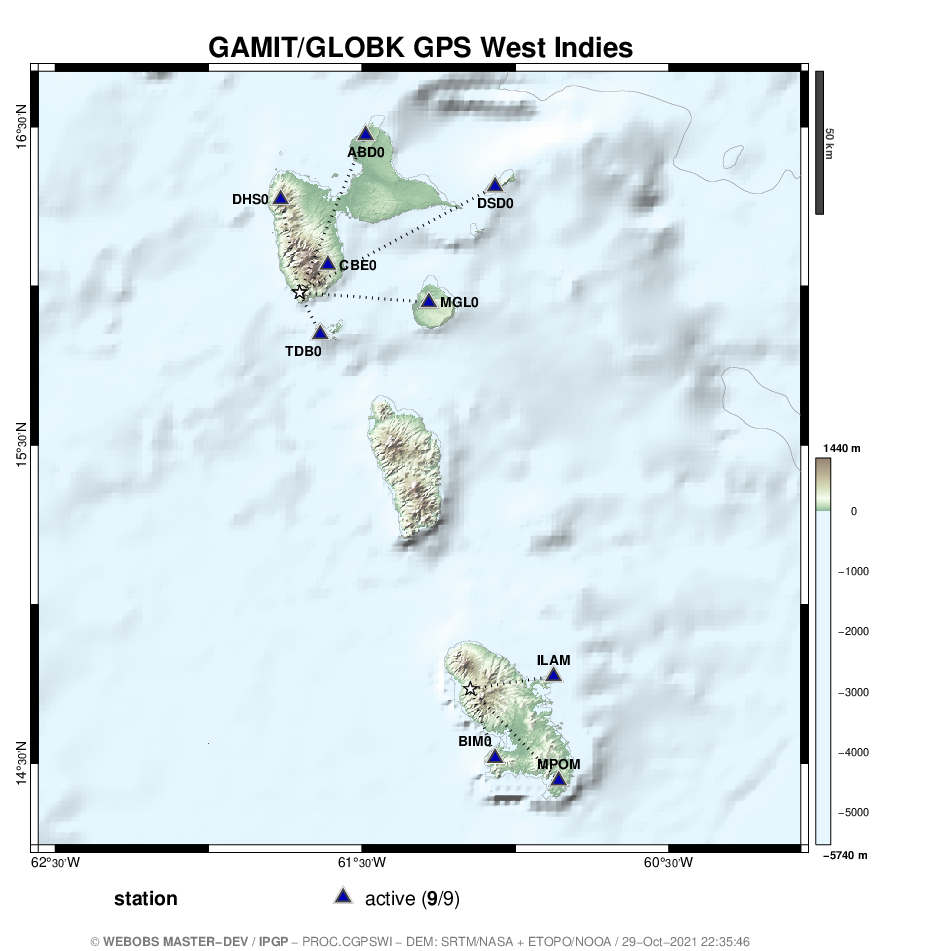
\includegraphics[height=.6\textwidth]{figures/PROC_CGPSWI_map.png}
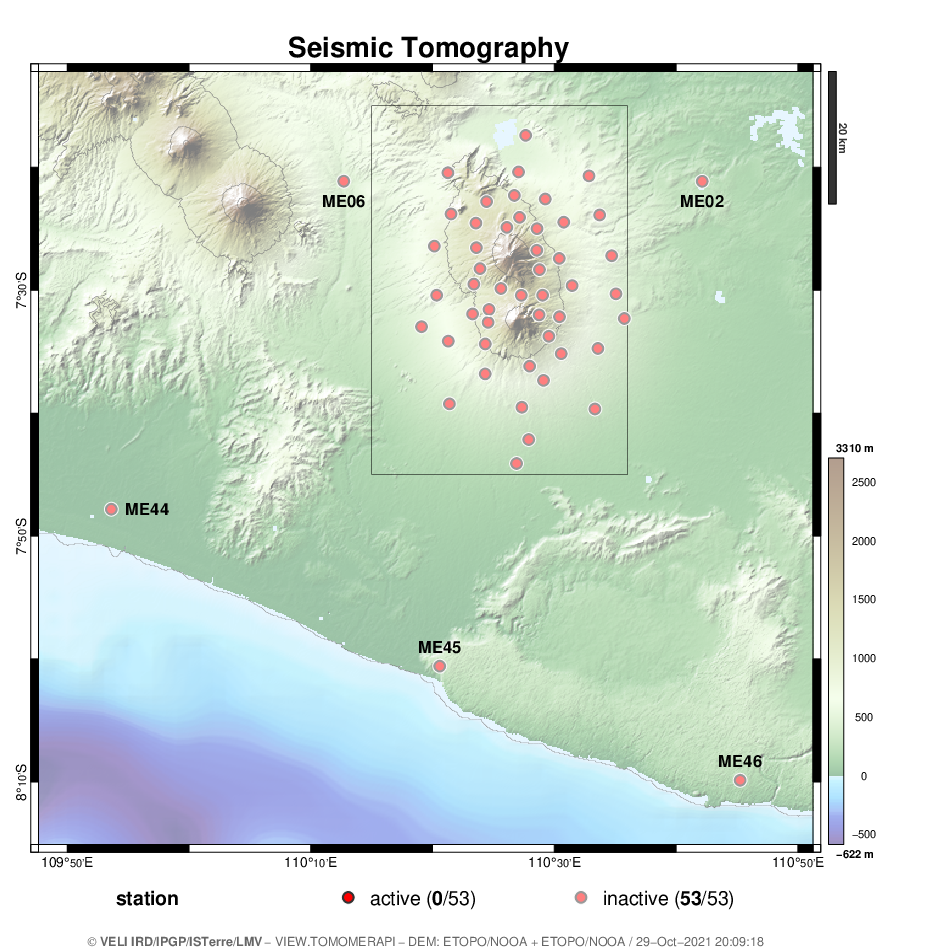
\includegraphics[height=.6\textwidth]{figures/VIEW_TOMOMERAPI_map.png}
\caption{Examples of GRID's maps created by GRIDMAPS.}
\end{figure}

% - - - - - - - - - - - - - - - - - - - - - - - - - - - - - - - - -
\subsubsection{Configuration}

Each \wo{grid} map is depending on two configuration files: one is common for all grids to define the basemap parameters:

\lstinputlisting[title=\wofile{GRIDMAPS.rc}]{../../SETUP/CONF/GRIDMAPS.rc}

and the other is the configuration file of the \wo{grid} itself to define the parameters associated to \wo{nodes} (see for example the \wo{view} example in section \ref{views}).

% - - - - - - - - - - - - - - - - - - - - - - - - - - - - - - - - -
\subsubsection{Activation}

GRIDMAPS is set by default when installing \webobs. It should be active at the first scheduler start. Parameters are as follows:

\begin{tabular}{rl}
\textbf{jid:}      & gridmaps \\
\textbf{res:}      & gridmaps \\
\textbf{xeq1:}     & \$WEBOBS\{JOB\_MCC\} gridmaps \\
\textbf{interval:} & 86400 \\
\textbf{logpath:}  & gridmaps \\
\textbf{valid:}    & Y \\
\end{tabular}

You may check if it runs correctly in the Scheduler Runs page (see Section \ref{scheduler}).


% -----------------------------------------------------------------
\subsection{LOCASTAT}
\label{locastat}

\begin{figure}
\includegraphics[width=\textwidth]{figures/IAIOBSPC01_map.png}
\caption{Example of NODE's map created by LOCASTAT.}
\end{figure}

The location map appears in each \wo{node} page if coordinates are defined. The map is automatically made and updated by LOCASTAT application. Maps are updated when the map timestamp is older than \wo{node}'s configuration file. So to force the update of a location map, you may modify any parameter in the \wo{node} configuration, typically the coordinates values or positioning date. 

The map contains 4 maps at different scales, all centered on the \wo{node} position, from left to right with a progressive zoom effect. Basemaps are built from the free worldwide topography data SRTM~\footnote{see \url{http://www2.jpl.nasa.gov/srtm/}} and specific colormap and rendering methods. It is possible to specify a user-defined DEM (Digital Elevation Model) for the highest resolution scale map (right frame).


\lstinputlisting[title=\wofile{LOCASTAT.rc}]{../../SETUP/CONF/LOCASTAT.rc}


% ==================================================================
\section{SEFRAN3/MC3: seismic chart and bulletin}

% -----------------------------------------------------------------
\subsection{Overview}

The SEFRAN3 is a graphical interface to operate seismic data flux, manual and semi-automatic detection of events, and earthquake catalog bulletin management.

The name ``SefraN'' is a contraction of \textit{Sefram Numérique}; it comes from a 70's paper strip-chart recording instrument from the French factory \textit{SEFRAM\textregistered}, used during decades in French observatories. Starting 2001, the system has been replaced by a numerical simulation using local data files archives in SUDS format. SEFRAN3 is the third version of SefraN which now uses data flow from SeedLink protocol.

A second tool called ``Main Courante'' hereafter named MC3, is a database of seismic events that is linked to SEFRAN3 interface and possibly to external earthquake catalogs like a local SeisComP3 or any FDSN-webservice compatible database like EMSC or USGS.

The SEFRAN3 works with a fixed selection of channels (up to 15) coming from a single server source, that will be displayed together as time series using 2 different time scales (normal and high) that simulate the paper speed. SEFRAN3 has 4 different GUI:
\begin{enumerate}

\item Main page showing hourly thumbnail images of seismic signals for a given period of time. Identified events are shown as overlaying colored tags. Bottom part of the page is showing realtime state of each channel with some statistics on the data quality. There is two display modes:
\begin{itemize}
\item real-time automatic refreshing page, for the last X hours/days of data;
\item any date selection for one or more days.
\end{itemize}

\item One hour display of full-resolution image in a wide window that can be spanned and scrolled through time.

\item A form showing a single event at high-speed time resolution of seismic signals, with possibility of editing data and submitting to the database.

\item A detailed table of events list with date selection, filters, and dynamic graphs.

\end{enumerate}

\textbf{Notice:} SEFRAN3 is using extensively the network connection (for data flux) and external programs like \wofile{arclink\_fetch} (from \textit{SeisComP3}), \wofile{slinktool} (from \textit{IRIS}) and \wofile{convert} (from \textit{ImageMagick}). If you experience any trouble, check first the network, the data availability on servers, and the third-party programs. You might add the variable \wokey{DEBUG|Y} in the configuration file to make the logs more verbose.

% -----------------------------------------------------------------
\subsection{SEFRAN3 installation}


\begin{figure}
\includegraphics[width=\textwidth]{figures/sefran3_diagram.pdf}
\caption{Schematic diagram of SEFRAN3 main parameters.}
\label{sefran3_diagram}
\end{figure}

SEFRAN3 is based on 1-minute images of seismic traces. It works within a loop that will end after a minimum duration run. Each loop will scan the existing images on disk, and make new images (real-time first, then look at older periods for gaps) or update them using broom wagons that check the data completeness after some time delay. There is also a short delay of few seconds to take into account the data flux lateness from real-time, and a longer delay to switch from SeedLink data request (convenient for real-time data flux) to ArcLink data request (convenient for archived data). Figure \ref{sefran3_diagram} is a summary of main parameters.


% - - - - - - - - - - - - - - - - - - - - - - - - - - - - - - - - -
\subsubsection{Configuration files}

To configure a new SEFRAN3, copy the template files \wofile{SEFRAN3.conf} and \wofile{SEFRAN3\_Channels.conf} to, for example, \wofile{MYSEFRAN.conf} and \wofile{MYSEFRAN\_Channels.conf}.


\wofile{MYSEFRAN\_Channels.conf} file sets the channel list. Each channel is defined by its alias (a short code used for display), the stream string (used for the data request), the sensitivity factor (to convert counts to m/s), the filter (median, trend or spline removal), the peak-to-peak signal amplitude, and the color. A good conduct is to order the channels from North to South, and give different colors for specific regions. There is no limit to the number of channels, but a maximum of 15 channels is recommended for a normal screen resolution.

\wofile{MYSEFRAN.conf} file is the main configuration file. It defines a lot of things like output paths, server address and all parameters of graphical outputs and SEFRAN3 behavior.

\lstinputlisting[title=\wofile{SEFRAN3\_Channels.conf}]{../../SETUP/CONF/SEFRAN3_Channels.conf}

\lstinputlisting[title=\wofile{SEFRAN3.conf}]{../../SETUP/CONF/SEFRAN3.conf}


% - - - - - - - - - - - - - - - - - - - - - - - - - - - - - - - - -
\subsubsection{Activation}

To activate the SEFRAN3, add a new job in the scheduler, for example with following parameters:

\begin{tabular}{rl}
\textbf{jid:}      & mysefran \\
\textbf{res:}      & mysefran \\
\textbf{xeq1:}     & \$WEBOBS\{JOB\_MCC\} sefran3 \\
\textbf{xeq2:}     & MYSEFRAN \\
\textbf{interval:} & 600 \\
\textbf{logpath:}  & mysefran \\
\textbf{valid:}    & Y \\
\end{tabular}

After activation, check that it runs correctly in the Scheduler Runs page (see Section \ref{scheduler}).

To access the main SEFRAN3 page, use the following URL (can be set for instance in the menu bar):

\wocmd{/cgi-bin/sefran3.pl?header=1\&s3=MYSEFRAN}

Further options are available to access all display possibilities. See \wocmd{perldoc CODE/cgi-bin/sefran3.pl}.


% -----------------------------------------------------------------
\subsection{MC3 configuration}

\lstinputlisting[title=\wofile{MC3.conf}]{../../SETUP/CONF/MC3.conf}

\lstinputlisting[title=\wofile{MC3\_Codes.conf}]{../../SETUP/CONF/MC3_Codes.conf}

%\lstinputlisting[title=\wofile{MC3\_Headers.conf}]{../../SETUP/CONF/MC3_Headers.conf}

\lstinputlisting[title=\wofile{MC3\_Amplitudes.conf}]{../../SETUP/CONF/MC3_Amplitudes.conf}

\lstinputlisting[title=\wofile{MC3\_Durations.conf}]{../../SETUP/CONF/MC3_Durations.conf}


% -----------------------------------------------------------------
\subsection{Links with earthquake event catalogs}

% - - - - - - - - - - - - - - - - - - - - - - - - - - - - - - - - -
\subsubsection{SeisComP3}

% - - - - - - - - - - - - - - - - - - - - - - - - - - - - - - - - -
\subsubsection{EarthWorm}



% ==================================================================
\section{GENPLOT: generic time series}
\label{genplot}

% -----------------------------------------------------------------
\subsection{Overview}

GENPLOT is the default superproc to plot time series from any source of data, particularly the time series formats (see section \ref{timeseries}). GENPLOT is able to produce graphics and text outputs from data channels of associated NODES. All the outputs will be processed for a list of preset time scales, which can be any of the following:
\begin{itemize}
\item a fixed duration (expressed in hour, day, week, month or year) until the present time (moving window);
\item a window from a reference date until present time (extending window);
\item all available data.
\end{itemize}

GENPLOT will produce, for each time scale:
\begin{itemize}
\item one graph per \wo{node} showing separated subplot for each selected channel;
\item one summary graph combining all \wo{nodes} on each channel subplot using different colors.
\end{itemize}

The plotted channels for the per-node and summary graphs are both configurable
using respectively \wo{NODE\_CHANNELS} and \wo{SUMMARY\_CHANNELS}. Titles and
line and marker style can also be configured:
\begin{itemize}
\item set \wo{PERNODE\_TITLE} and/or \wo{SUMMARY\_TITLE} to customize the title;
\item set \wo{PERNODE\_LINESTYLE} and/or \wo{SUMMARY\_LINESTYLE} to a line specification string, a combination of two components:
	\begin{itemize}
		\item a line type (see possible values in table \ref{linestyle}),
		\item a marker symbol type (see possible values in table \ref{markertype}),
	\end{itemize}
 to choose between drawing markers and/or line and define their style; note you might specify a marker only with no line, then only the markers are plotted;
\item the line width and marker size can be different for each time scale using
  respectively \wo{LINEWIDTHLIST} and \wo{MARKERSIZELIST}, that should both
  define a size to use (in \texttt{pt}) for each of the timescales defined in
  \wo{TIMESCALELIST}, coma separated values;
\item colors are chosen automatically by the proc: for the summary graph it will be one color per node, for the per-node graph it will be one color per channel.
\end{itemize}

% -----------------------------------------------------------------
\subsection{Configuration}

Some parameter keys of GENPLOT are common for all \wo{procs} and \wo{grids} so are identical with the \wo{view} configuration (see section \ref{views}).

\lstinputlisting[title=\wofile{GENPLOT template}]{../../CODE/tplates/PROC.DEFAULT}

% - - - - - - - - - - - - - - - - - - - - - - - - - - - - - - - - -
\subsubsection{Time scales}



% ==================================================================
\section{HYPOMAP: Earthquake hypocenter maps from seismic catalog}

% -----------------------------------------------------------------
\subsection{Overview}

% -----------------------------------------------------------------
\subsection{Configuration}

Some parameter keys of HYPOMAP are common for all \wo{procs} and \wo{grids} so are identical with the \wo{view} configuration (see section \ref{views}).

\lstinputlisting[title=\wofile{HYPOMAP template}]{../../CODE/tplates/PROC.HYPOMAP}


% ==================================================================
\section{HELICORDER: Seismic helicorder}

% -----------------------------------------------------------------
\subsection{Overview}

% -----------------------------------------------------------------
\subsection{Configuration}

Some parameter keys of HELICORDER are common for all \wo{procs} and \wo{grids} so are identical with the \wo{view} configuration (see section \ref{views}).

\lstinputlisting[title=\wofile{HELICORDER template}]{../../CODE/tplates/PROC.HELICORDER}


% ==================================================================
\section{RSAM: Realtime Seismic Amplitude Measurement}

% -----------------------------------------------------------------
\subsection{Overview}

% -----------------------------------------------------------------
\subsection{Configuration}

Some parameter keys of RSAM are common for all \wo{procs} and \wo{grids} so are identical with the \wo{view} configuration (see section \ref{views}).

\lstinputlisting[title=\wofile{RSAM template}]{../../CODE/tplates/PROC.RSAM}


% ==================================================================
\section{GNSS: GPS time series, vectors and modelling}

% -----------------------------------------------------------------
\subsection{Overview}

% -----------------------------------------------------------------
\subsection{Configuration}

Some parameter keys of GNSS are common for all \wo{procs} and \wo{grids} so are identical with the \wo{view} configuration (see section \ref{views}).

\lstinputlisting[title=\wofile{GNSS template}]{../../CODE/tplates/PROC.GNSS}


% ==================================================================
\section{EXTENSO: Extensometry time series and vectors}

% -----------------------------------------------------------------
\subsection{Overview}

% -----------------------------------------------------------------
\subsection{Configuration}

Some parameter keys of EXTENSO are common for all \wo{procs} and \wo{grids} so are identical with the \wo{view} configuration (see section \ref{views}).

\lstinputlisting[title=\wofile{EXTENSO template}]{../../CODE/tplates/PROC.EXTENSO}


% ==================================================================
\section{TILT: Tiltmetry time series, vectors and modelling}

% -----------------------------------------------------------------
\subsection{Overview}

% -----------------------------------------------------------------
\subsection{Configuration}

Some parameter keys of TILT are common for all \wo{procs} and \wo{grids} so are identical with the \wo{view} configuration (see section \ref{views}).

\lstinputlisting[title=\wofile{TILT template}]{../../CODE/tplates/PROC.TILT}


% ==================================================================
\section{METEO: meteorological time series}

% -----------------------------------------------------------------
\subsection{Overview}

% -----------------------------------------------------------------
\subsection{Configuration}

Some parameter keys of METEO are common for all \wo{procs} and \wo{grids} so are identical with the \wo{view} configuration (see section \ref{views}).

\lstinputlisting[title=\wofile{METEO template}]{../../CODE/tplates/PROC.METEO}


% ==================================================================
\section{WATERS: chemical analysis}

% -----------------------------------------------------------------
\subsection{Overview}

% -----------------------------------------------------------------
\subsection{Configuration}

Some parameter keys of WATERS are common for all \wo{procs} and \wo{grids} so are identical with the \wo{view} configuration (see section \ref{views}).

\lstinputlisting[title=\wofile{WATERS template}]{../../CODE/tplates/PROC.WATERS}



% ==================================================================
\section{PROCS graph and data request}

% -----------------------------------------------------------------
\subsection{Overview}

A dedicated form \wocmd{/cgi-bin/formREQ.pl} allows to make user request to get any outputs (graphs and data) from PROCS sharing the same set of time span and parameters, mostly independent from the SCHEDULER's jobs. The identified USER has to be authorized for reading on the PROC to perform a request on it.

\includegraphics[width=\textwidth]{figures/formREQ.png}

% -----------------------------------------------------------------
\subsection{Description}

The form presents a list of available PROCS with empty check boxes. One or more PROCS can be selected, in that case a parameter list might appear for each of selected PROC, allowing the user to change the values. Please note there is no validity check of the values so a request may fail in case of invalid fields.

The main parameter to define is the date and time span: \textbf{Start date} and \textbf{End date} with time. Default is the last full month. A list of preset dates is also available. The date and time must be in UT. 

Also some output parameters can be defined:
\begin{itemize}
\item \textbf{TZ:} the output time zone, in hours. Will affect graphs and data exports.
\item \textbf{Date format:} the format of dates for time series plots axis ticks label.
\item \textbf{Cumulate:} time for cumulating data (when cumulative allowed in the PROC), in day. Use fraction or any arithmetic formula if needed.
\item \textbf{Decimate:} number of sample for decimation of the raw data (time series).
\item \textbf{Marker size:} maker size in points (if the PROC uses markers).
\item \textbf{Line width:} line width in points (if the PROC uses lines).
\item \textbf{PPI:} resolution for PNG output images, in pixel per inch.
\item \textbf{Postscript:} outputs the EPS vector graphic images (default is cheched).
\item \textbf{PDF:} outputs a PDF version of images.
\item \textbf{Exports:} outputs data (text files or others depending on the PROC).
\end{itemize}

After submit the request, each of the PROC will be submitted to SCHEDULER as specific jobs. The name of the job is made from date and time of the request, hostname and user login name.

The run of each PROC can be followed on the scheduler runs page. If a job ends with success, a notification email is sent to the user through the POSTBOARD. The email provides two links: a first to access the request results (graphs and exports) through a web interface similar to the routine PROC graphs. The second link allows to download a .tgz archive containing all images and files of the request.

A dedicated page is also available to access request results: \wocmd{/cgi-bin/showREQ.pl}. The page will show the user's requests and results (if the request job has ended successfully), or all the existing requests for ADMIN users.


% -----------------------------------------------------------------
\subsection{Configuration}

\begin{lstlisting}[title=\wofile{PROC.conf} (excerpt)]
SUBMIT_COMMAND|$WEBOBS{JOB_MCC} genplot $SELFREF -
SUBMIT_RESOURCE|myproc
REQUEST_KEYLIST|NAME,SUMMARY_RELATIVE,PERNODE_LINESTYLE
\end{lstlisting}

The request form displays any PROC containing a not-empty \wokey{SUBMIT\_COMMAND} parameter in its configuration. This parameter is the routine execution command line, ie. equivalent to the value of a XEQ1 in the SCHEDULER (see scheduler.pl doc) and, as such,
supporting \wo{\$WEBOBS} parameters substitution.

The \wokey{SUBMIT\_RESOURCE} is the optional routine execution mutex name (process lock) of as defined in SCHEDULER if the PROC is one of the routine jobs. This is to avoid possible conflicts of simultaneous runs.

Optionally, the \wokey{REQUEST\_KEYLIST} parameter is used to specify a list of comma-separated keys of existing parameters, that will be
presented to the user so that (s)he will have a chance to overwrite corresponding values for request execution.

The user defined output parameters \textbf{Date format}, \textbf{Cumulate}, \textbf{Decimate}, \textbf{Marker size} and \textbf{Line width} correspond to table values \wokey{DATESTRLIST}, \wokey{CUMULATELIST}, \wokey{DECIMATELIST}, \wokey{MARKERSIZELIST} and \wokey{LINEWIDTHLIST}, respectively.

The list of available preset values for PPI resolution, marker size and line width can be defined in \wofile{WEBOBS.rc} :

\begin{lstlisting}[title=\wofile{WEBOBS.rc} (excerpt)]
REQ_PPI_LIST|75,100,150,300,600
REQ_MARKERSIZE_LIST|1,2,4,6,10,15,20
REQ_LINEWIDTH_LIST|0.1,0.25,0.5,1,1.5,2,3
\end{lstlisting}

To use the notification email facility, POSTBOARD must be running, and the special event \textbf{formreq.} must be defined and valid (see \webobs Users Manager page).



% ==================================================================
\section{Data formats available for PROCS}

Formats are defined for a whole PROC in the \wokey{RAWFORMAT} PROC's variable, or for individual NODE in the \wokey{RAWFORMAT} NODE's parameter which overwrites the PROC value. The \wokey{RAWDATA} PROC's variable can be defined for all associated NODES, and any individual NODE's \wokey{RAWDATA} may overwrite it. A special variable \wocmd{\$FID} might be used and will be replaced by each NODE's value. For most of the formats, the Calibration File of each associated NODE will define the list of available channels and associated parameters.

See the source codes \wofile{CODE/matlab/readfmtdata.m} help for more details.

% -----------------------------------------------------------------
\subsection{Waveforms formats}

These formats are standards in seismology for waveforms data, but they are also used for other types of geophysical sensors. The standards use local files in specific format or dedicated protocol request from distant servers. Particularly, the full channel stream must be defined for each NODE, i.e.:

\begin{tabular}{ccl}
NET & network code & \wokey{FDSN\_NETWORK\_CODE} NODE's parameter\\
STA & station code & \wokey{FID} NODE's parameter\\
CHA & channel code & calibration file ``Chan. Code'' channel parameter\\
LOC & location code & calibration file ``LC'' channel parameter\\
\end{tabular}


% - - - - - - - - - - - - - - - - - - - - - - - - - - - - - - - - -
\subsubsection{\{miniseed\}: miniSEED files}
\label{miniseed}

Single of multiple local files in miniSEED format. \wokey{RAWDATA} defines the filename(s) using standard bash syntax (accepts wildcards). Some limitations may apply due to bash line size limit.


% - - - - - - - - - - - - - - - - - - - - - - - - - - - - - - - - -
\subsubsection{\{seedlink\}: SeedLink request}
\label{seedlink}

SeedLink protocol request from a distant or local server. \wokey{RAWDATA} defines the server with \wocmd{host:port}. The format uses external program \wocmd{slinktool} defined by the \wofile{WEBOBS.rc} \wokey{SLINKTOOL\_PRGM} parameter. \wokey{DATALINK\_DELAY\_SECONDS} defines the delay in seconds from real-time for the last data.


% - - - - - - - - - - - - - - - - - - - - - - - - - - - - - - - - -
\subsubsection{\{arclink\}: SeisComP3 ArcLink request}
\label{arclink}

ArcLink protocol request from a distant or local server. \wokey{RAWDATA} defines the server with \wocmd{host:port}. Optional parameter \wokey{ARCLINK\_USER} can be defined (default user is 'wo'). The format uses external program \wocmd{arclink\_fetch} defined by the \wofile{WEBOBS.rc} \wokey{ARCLINKFETCH\_PRGM} parameter.

% - - - - - - - - - - - - - - - - - - - - - - - - - - - - - - - - -
\subsubsection{\{combined\}: SeisComP3 combined SeedLink/ArcLink request}

The combined format will use SeedLink protocol for recent data and ArcLink protocol for data older than a delay. \wokey{RAWDATA} must contain the string \wocmd{seedlinkhost:seedlinkport;arclinkhost:arclinkport;delayhours}. It will use both external programs defined in \wofile{WEBOBS.rc} \wokey{SLINKTOOL\_PRGM} and \wokey{ARCLINKFETCH\_PRGM} parameters.

% - - - - - - - - - - - - - - - - - - - - - - - - - - - - - - - - -
\subsubsection{\{fdsnws-dataselect\}: FDSN web-service dataselect request}

Distant waveform request using the FDSN web-service protocol available at most of seismological data centers. \wokey{RAWDATA} must contain the base URL, for example: \wocmd{http://service.iris.edu/fdsnws/dataselect/1/query?} for IRIS.

% - - - - - - - - - - - - - - - - - - - - - - - - - - - - - - - - -
\subsubsection{\{winston\}: EarthWorm Winston wave server request}

EarthWorm Winston wave server (WWS) protocol request from a distant or local server. \wokey{RAWDATA} defines the server with \wocmd{host:port}.


% -----------------------------------------------------------------
\subsection{Generic time series}
\label{timeseries}

These formats will return time series of data channels, like the waveform formats do but usually the data sampling frequency is lower than for seismic waveforms, so it can be managed using data files stored in local directories. Number of channels depends on the data and can be selected and calibrated using the NODE's calibration file.

% - - - - - - - - - - - - - - - - - - - - - - - - - - - - - - - - -
\subsubsection{\{ascii\}: Generic ASCII text files}

Attempt to read generic text files with regular data columns. \wokey{RAWDATA} contains the full path and filename(s) using bash wildcard facilities. The data files must be organized as regular columns of numbers (strings will produce a column of NaN), any separator character, and the date and time must be defined as 3 (year, month, day) or 6 columns (year, month, day, hour, minute, second) at some place (default is the 6 first columns). If there is no calibration file for a NODE, the header line will be used to get the channel names.

For this format you may define optional additional \wokey{FID\_*} keys for each NODE to specify the format:

\begin{tabular}{rl}
\wokey{FID\_FS} & field separator character (default is semicolumn),\\
\wokey{FID\_TIMECOLS} & index vector of columns defining date\&time in order: year month day hour minute second,\\
\wokey{FID\_NF} & number of data columns in the file, considering all non-numeric as separator (default is automatic),\\
\wokey{FID\_HEADERLINES} & number of header lines (default is 1).
\end{tabular}


\begin{lstlisting}[language={},title=Generic ASCII format example 1: time + data channels 1 to 3.]
               Date;                   P_0;                 SO2_0;                 H2S_0;
06/06/2017 18:00:00;            752.579529;             -0.061299;             -0.031172;
06/06/2017 18:00:09;            724.445852;             -0.071515;             -0.024938;
\end{lstlisting}

\begin{lstlisting}[title=\wokey{FID\_*} parameters to read example 1 file.]
FID_FS|;
FID_TIMECOLS|3,2,1,4,5,6
FID_NF|9
FID_HEADERLINES|1
\end{lstlisting}


\begin{lstlisting}[language={},title=Generic ASCII format example 2: data channel 1 (all NaN) + time + data channels 2 to 4.]
VMAB    01/01/12        06:20:11        132     338     40.6
VMAB    01/01/12        06:40:11        135     337     40.7
VMAB    01/01/12        07:00:11        133     336     40.6
\end{lstlisting}


\begin{lstlisting}[title=\wokey{FID\_*} parameters to read example 2 file.]
FID_FS|\t
FID_TIMECOLS|4,3,2,5,6,7
FID_NF|10
FID_HEADERLINES|0
\end{lstlisting}


% - - - - - - - - - - - - - - - - - - - - - - - - - - - - - - - - -
\subsubsection{\{sql-table\}: SQL-table request}

Request to a SQL database using external program \wocmd{mysql}. \wokey{RAWDATA} must contain the full command that will return the data in the text format \wocmd{yyyy-mm-dd HH:MM:SS data1 data2 data3 ...}. The command must include two variables \wocmd{\$date1} and \wocmd{\$date2} that will be replaced by the timespan request. Example:

\wocmd{mysql -h host -u user -ppasswd -Ddatabase -N -B -e 'SELECT time,data1,data2,data3 from \$FID WHERE time between "\$date1" and "\$date2";'}

will make a request from the \wocmd{database} at server \wocmd{host} on the table \wocmd{\$FID} and return timestamp and data columns. The calibration file must define these 3 channels in that order.

% - - - - - - - - - - - - - - - - - - - - - - - - - - - - - - - - -
\subsubsection{\{cr10xasc\}: Campbell Scientific CR10X ASCII files}

Daily data files from data loggers CR10X archived in a specific directory structure. \wokey{RAWDATA} contains the main directory path, in which files are stored in the following subpath and name: \wocmd{FID/YYYY/YYYYMMDD.DAT}. Each file has the data format: \wocmd{PRGM,yyyy,doy,HM,data1,data2, ... ,dataN}, where \wocmd{PRGM} is the program number, \wocmd{yyyy} the 4-digit year, \wocmd{doy} the day of the year (ordinal day), \wocmd{HM} the hour and minute with leading blanks, and the data.

\begin{lstlisting}[language={},title=Campbell CR10X format example]
121,2013,365,2340,8.6971,-20.168,0,91.3,22.48,0,826.42,12.514,99999,0,0
121,2013,365,2350,8.7294,-20.016,0,88.4,20.02,0,826.43,12.521,99999,0,0
\end{lstlisting}


% - - - - - - - - - - - - - - - - - - - - - - - - - - - - - - - - -
\subsubsection{\{t0a5\}: Campbell Scientific T0A5 ASCII files}

Daily data files from Campbell Scientific data loggers in the T0A5 output format, archived in a specific directory structure. \wokey{RAWDATA} contains the main directory path, in which files are stored in the following subpath and name: \wocmd{FID/YYYY/FIDYYYYDDD.DAT}. Each file has the data format: \wocmd{"yyyy-mm-dd HH:MM:SS",data1,data2, ... ,dataN}.

\begin{lstlisting}[language={},title=Campbell T0A5 format example]
"2014-01-11 00:00:00",68148,12.1,16.07,15.29,100,938,0.02,0.02,0,7.875425,98.67353,10.86884,0,0,0,0,0,0,0,0
"2014-01-11 00:10:00",68149,12.1,15.96,14.76,100,938,0.021,0.021,0,7.200668,101.9742,11.35311,0,0,0,0,0,0,0,0
\end{lstlisting}


% - - - - - - - - - - - - - - - - - - - - - - - - - - - - - - - - -
\subsubsection{\{porkyasc\}: USGS Porky ASCII files}

Daily data files from USGS Porky data systems, archived in a specific directory structure. \wokey{RAWDATA} contains the main directory path, in which files are stored in the following subpath and name: \wocmd{FID/YYYY/YYYYMMDD.DAT}. Each file has the data format: \wocmd{DD-MMM-YYYY HH:MM data1 data2 ... dataN}.

\begin{lstlisting}[language={},title=USGS Porky format example]
01-JAN-2014 00:00  00000  00029  00013  03181  00001 -00998 -00998 -00998
01-JAN-2014 00:05  00001  00040  00010  03182  00001 -00998 -00998 -00998
\end{lstlisting}

% -----------------------------------------------------------------
\subsection{Quakes catalogs}

These are specific formats for PROCS dedicated to earthquake catalogs. These formats returns a list of event with preset channels, like Latitude, Longitude, Depth, Magnitude, etc... There is no calibration file (if it exists it will be ignored). It is possible to link this format with a Main Courante (MC3) database using the NODE's \wokey{FID\_MC3} with the MC3 name. In that case some information from MC3 might be associated to identified events.

An other specificity of these formats is that all catalogs from different associated NODES will be concatenated in a single data matrix. This allows to merge for instance, a distance worldwide catalog like USGS (for large earthquakes), a local catalog from a local network, and an historical catalog in an old-fashion file format.

% - - - - - - - - - - - - - - - - - - - - - - - - - - - - - - - - -
\subsubsection{\{hyp71sum2k\}: Quake Hypo71 summary lines year 2000 compatible}

Single file in the HYPO71 ASCII format identified by \wokey{RAWDATA} with full filename and path. The standard format is completed by two last columns: \wocmd{SCode} for a 5-letter identification code, and \wocmd{File} for the waveform filename. Note the file is column formatted, without any delimiter, there is no leading zeros but blanks, and the longitude value is positive towards the West.

\begin{lstlisting}[title=HYPO71 format example]
#   DATE ORIGIN     LAT_N     LON_W     DEPTH    MAG NO GAP DMIN  RMS  ERH  ERZ Q  SCode File
18430208 1440 00.00 16-44.00  61-10.00 000.00   8.00 00 000 00.0 0.00 00.0 00.0 0  TE9GM
20141005 1819 07.34 14-48.70  61-10.33  -0.24 D 1.52  8 166  0.3 0.26  0.6  0.8 C  EB1   20141005_181900.mq0
\end{lstlisting}


% - - - - - - - - - - - - - - - - - - - - - - - - - - - - - - - - -
\subsubsection{\{fdsnws-event\}: Quake FDSN WebServices event request}

Distant event data request using the FDSN web-service protocol available at most of seismological data centers. It accepts the QuakeML 1.2 format only. \wokey{RAWDATA} must contain the base URL, for example: \wocmd{http://service.iris.edu/fdsnws/event/1/query?} for IRIS.


% - - - - - - - - - - - - - - - - - - - - - - - - - - - - - - - - -
\subsubsection{\{scevtlog-xml\}: Quake SeisComP3-xml files}

Reads a files architecture created by the SeisComP3 scevtlog module. \wokey{RAWDATA} defines the path root where events are stored in a subdirectory structure as \wofile{YYYY/MM/DD/eventID/eventID.last.xml} in the SC3ML format.


% -----------------------------------------------------------------
\subsection{GNSS solutions}

These are specific formats for PROCS dedicated to positioning data from GNSS (Global Network Satellite Systems) like GPS or GLONASS. These formats returns preset channels: Eastern, Northern, Vertical and Orbit type.

% - - - - - - - - - - - - - - - - - - - - - - - - - - - - - - - - -
\subsubsection{\{gipsy-tdp\}: JPL GIPSY-OASIS TDP files}

TDP (Time Dependant Parameter) files results of the JPL GIPSY-OASIS processing in IRTF. The format uses only the position part of the data: \wocmd{Time   Dinit   Dfinal error STA c ssss} where Time is GPS date in seconds past J2000, \wocmd{c} is the component in geocentric referential, \wocmd{ssss} the station name. \wokey{P.RAWDATA} contains the path root directory where daily solutions files are stores in a subdirectory structure as \wofile{FID/YYYY/FID/YYYY-MM-DD.FID.tdp*}.

\begin{lstlisting}[language={},title=GIPSY-OASIS TDP format example]
 476712000.0000   1797.11460400000       1797.11463384421      9.751E-07  STA Z   ABD0
 476712000.0000  -5375.91966100000      -5375.91974126823      2.297E-06  STA Y   ABD0
 476712000.0000   2920.34971800000       2920.34975977472      1.377E-06  STA X   ABD0
\end{lstlisting}


% - - - - - - - - - - - - - - - - - - - - - - - - - - - - - - - - -
\subsubsection{\{globkval\}: MIT GAMIT-GLOBK VAL files}

Single file output of Gamit-GlobK processing in ITRF referencing. \wokey{P.RAWDATA} defines the full path filename of the .VAL result file which contains solution timeseries for each component and each station.

\begin{lstlisting}[language={},title=GAMIT-GLOBK VAL format example]
 Combination of ALL networks
ILAM_GPS to E Solution  1 +  32197594.810 m

 2012 12 19 11 59  32197594.80990    0.00626   -0.00183   0.00626
 2012 12 20 11 59  32197594.81087    0.00433   -0.00090   0.00433
 ...
 2013 12 17 11 59  32197594.81866    0.00519   -0.00799   0.00519

Wmean   32197594.8184 m +- 0.0003 from  340 data. WRMS   5.2 mm, NRMS  1.19
Slope    15.01 +-     0.84 mm/yr, WRMS   3.1 mm, NRMS  0.70, dur  0.99 <> 2013.41 yr

 Combination of ALL networks
ILAM_GPS to U Solution  1 +        -0.750 m

 2012 12 19 11 59        -0.74977    0.01910    0.01410   0.01910
 2012 12 20 11 59        -0.74919    0.01048    0.01471   0.01048
 ...
 2013 12 17 11 59        -0.80060    0.01370   -0.02614   0.01370

Wmean         -0.7686 m +- 0.0006 from  340 data. WRMS   9.3 mm, NRMS  0.82
Slope   -10.66 +-     2.20 mm/yr, WRMS   8.8 mm, NRMS  0.78, dur  0.99 <> 2013.41 yr
\end{lstlisting}


% -----------------------------------------------------------------
\subsection{Other specific formats}

These formats are basically time series but the channels are predefined.

% - - - - - - - - - - - - - - - - - - - - - - - - - - - - - - - - -
\subsubsection{\{teqc-qc\}: TEQC Rinex quality check}

% - - - - - - - - - - - - - - - - - - - - - - - - - - - - - - - - -
\subsubsection{\{naqs-soh\}: NAQS State of Health}

% - - - - - - - - - - - - - - - - - - - - - - - - - - - - - - - - -
\subsubsection{\{wodbform\}: WebObs database forms}

This format is not selectable. It becomes active automatically when a PROC is associated to a FORM and its specific database. In that case the data columns are determined by the FORM type.


%%%%%%%%%%%%%%%%%%%%%%%%%%%%%%%%%%%%%%%%%%%%%%%%%%%%%%%%%%%%%%%%%%%%
%%%%%%%%%%%%%%%%%%%%%%%%%%%%%%%%%%%%%%%%%%%%%%%%%%%%%%%%%%%%%%%%%%%%
%\definecolor{charcoal}{rgb}{0.21, 0.27, 0.31}
\definecolor{charcoal}{gray}{0.30}
\lstdefinestyle{console}
{language=bash,
basicstyle=\scriptsize\ttfamily\color{white}\bfseries,
backgroundcolor=\color{charcoal},
keywordstyle=\color{white},
alsoletter={:~$},
}


\chapter{Administration}


% ==================================================================
\section{Users, Groups and Authorizations}

% -----------------------------------------------------------------
\subsection{Overview}

\webobs uses its own AUTHORIZATION system, in addition to the Apache Authentication system, to identify its HTTP USERS and
control their individual ACCESS-RIGHTS to \webobs RESOURCES (ie. logical entities refering to files, processes, html-pages, whatever). 

AUTHORIZATION system elements:
\begin{itemize}
\item    a USERS TABLE that further identifies the USERS defined in the Apache Authentication files (eg. .htpasswd),
\item    a GROUPS TABLE that merely defines groups of USERS, to simplify (reduce number of) access-rights definitions,     
\item    RESOURCES are fully identified as \textbf{resourceType.resourceName}, 
\item    RESOURCES TABLES are the \textbf{resourceType} tables containing their own \textbf{resourceName} descriptions, 
\item    a \textbf{resourceName} description defines the relationship \textbf{uid-or-gid has access-rights},
\item    Supported access-rights are:
\begin{itemize}
\item    \textbf{R} = 1  Read 
\item    \textbf{E} = 2  Edit = Read + Write
\item    \textbf{A} = 4  Admin = Edit + Create/Delete
\end{itemize}
\end{itemize}


% -----------------------------------------------------------------
\subsection{Users table and Groups table}
\label{usertable}

A \webobs USER is identified by its LOGIN (string) as also defined in the HTTP Authentication system. A row in  
the USERS TABLE further defines a USER with the following information: 

\begin{itemize}
\item   LOGIN
\item   FULLNAME, the user's name
\item   UID, a short identification string, usually the user's name initials, to be used for access-rights and other functionnal needs
\item   EMAIL, the email address (somebody@somewhere) used by the \webobs POSTBOARD system,
\item   VALIDITY, to determine if the user is able to access some resource or not.
\end{itemize}

Two special UIDs are reserved for system use: 
\begin{itemize}
\item   \textbf{?} to identify a GUEST user (granted to undefined users for temporary/limited access to \webobs), 
\item   \textbf{!} to identify the WEBOBS OWNER.
\end{itemize}

Records of the GROUPS TABLE associate UIDs to GROUP names (aka GID). A GID must starts with a '+' sign.
A USER may be a member of more than one GROUP. A USER inherits all access-rights defined for the GROUP(s) it belongs to. 

Four (4) special GROUPs are pre-defined in \webobs: \textbf{+ADMIN}, \textbf{+DUTY}, \textbf{+OBSERVER} and \textbf{+VISITOR}. They are initially used to  
define access-rights to \webobs built-in tools and/or applications. 

% -----------------------------------------------------------------
\subsection{Resource tables}

The fully qualified name of a \webobs RESOURCE is \textbf{resourceType.resourceName}.

There are five (5) resourceType tables: \textbf{authviews}, \textbf{authprocs}, \textbf{authforms}, \textbf{authwikis} corresponding to the base \webobs objects 
and \textbf{authmisc} for any additional, unclassified, resourceNames definitions. They are already populated with resourceNames related to \webobs built-in tools and applications.

The special resourceName '\textbf{*}' stands for ``all resourceNames of this resourceType''.

resourceNames are strings, defined and documented by the developers of the \webobs tools or applications.

% -----------------------------------------------------------------
\subsection{Managing Users and Authorizations}

The USERS ADMIN page \textbf{/cgi-bin/usersMgr.pl} (built-in tool), initially restricted to the +ADMIN group, is used to create/modify/delete user and resources definitions.

USERS and RESOURCE TABLES have customization variables in the main configuration file \wofile{WEBOBS.rc}:

\begin{lstlisting}[title=\wofile{WEBOBS.rc} (excerpt)]
SQL_DB_USERS|${ROOT_CONF}/WEBOBSUSERS.db
SQL_TABLE_USERS|users
SQL_TABLE_AUTHPROCS|authprocs
SQL_TABLE_AUTHVIEWS|authviews
SQL_TABLE_AUTHFORMS|authforms
SQL_TABLE_AUTHWIKIS|authwikis
SQL_TABLE_AUTHMISC|authmisc
SQL_TABLE_GROUPS|groups
SQL_DB_USERS_AUTOREGISTER|YES
\end{lstlisting}

% -----------------------------------------------------------------
\subsection{Developing with Users and Authorizations system}

The \textbf{WebObs::Users} perl module is the built-in interface to the USERS/AUTHORIZATIONS objects and functions system.
Detailed programming information can be found in its 'perldoc' documentation, such as:

\begin{itemize}
\item   global variables USERS, USERIDS and CLIENT
\item   the special 'path-like' specification for resourceNames
\item   functions: \textbf{allUsers, clientHasRead, clientHasEdit, clientHasAdm, listRNames}
\end{itemize}

Developers may add/define/use their own resourceName(s) for their specific needs.


% -----------------------------------------------------------------
\subsection{Adding a new user}

Registration of a new user is done in 3 steps:

\begin{enumerate}
\item new user must fill the form (see screenshot \ref{regform}) by connecting to WebObs interface and click 'Cancel' when asked to login. The data (with encrypted password) will be stored as a new pipe-separated line in the file \wofile{DATA/DB/reglog} and an e-mail will be sent to user and \webobs owner;
\item two alternatives depending on the value of \wokey{SQL\_DB\_USERS\_AUTOREGISTER} key:
	\begin{enumerate}
		\item if 'YES', then the new user will be automatically added in the database with validity 'N' and without any associated group. UID is made from initials of the full name, if necessary adding suffix number. The encrypted password will be automatically added into \wofile{CONF/htpasswd} apache file;
		\item if 'NO', administrator must add the user manually using Users Admin interface (see section \ref{usertable}), and add manually the encrypted password as a new line into the file \wofile{CONF/htpasswd};
	\end{enumerate}
\item for both alternatives, administrator must validate the new user, eventually modify its UID, and associate it to a group or add specific resource access authorization. This step must be conducted with care since it gives an access (or edit/admin) to all or part of \webobs resources.
\end{enumerate}


\begin{figure}
\center
\includegraphics[width=.5\textwidth]{figures/registration_form.png}
\caption{Registration form for new users.}
\label{regform}
\end{figure}


% ==================================================================
\section{PostBoard}

% -----------------------------------------------------------------
\subsection{Overview}

\webobs tools and applications may wish to send (email) alerting/warning/information messages to \webobs USERs when detecting 
special processing conditions or other events. Deciding who needs/wishes to receive such messages, and actually sending them, should be
as easy as possible from the developers point of view; furthermore, \webobs administrators should be able to easily filter/choose which users 
should receive what, based on operationnal needs, authorizations concerns, and even user's choice of being (or not being) alerted.

The \webobs POSTBOARD system (notifications/subscriptions) addresses these needs. Elements of POSTBOARD architecture: 

\begin{itemize}
\item   Tools and applications simply and unconditionnaly send identified messages (NOTIFICATIONS) to POSTBOARD
\item   NOTIFICATIONS basically look like "eventname\textbar senderId\textbar message" 
\item   POSTBOARD is a daemon that tries to match the eventname of the NOTIFICATIONS it receives against active SUBSCRIPTIONS that 
tell it what to do: either send a mail to a UID (or GID), or trigger a command, or both
\item   a SUBSCRIPTION is a row in the \webobs NOTIFICATIONS TABLE with the following fields:

\begin{tabular}{ll}
\textbf{eventname} & identifying the SUBSCRIPTION to match NOTIFICATIONS sent to POSTBOARD\\ 
\textbf{validity}  & indicating active/inactive              \\  
\textbf{uid}       & UID or GID to whom mail the NOTIFICATION\\
\textbf{subject}   & subject of the mail being sent          \\  
\textbf{attachment}& optional, path of a file to attach to mail \\
\textbf{action}    & optional, a command to be executed      \\  
\end{tabular}
\end{itemize}

% -----------------------------------------------------------------
\subsection{Event names}

Event names identify and associate NOTIFICATIONS to SUBSCRIPTIONS:  
\begin{itemize}
\item   eventname    = string[.[string]] 
\item   string.string is known as the \textbf{majorname.minorname} form of an event-name
\item   \textbf{majorname.minorname} identifies a single subscription named majorname.minorname AND  
\item   a \textbf{majorname.} subscription, if defined as such (don't forget the ending dot!), will also match all \textbf{majorname.minorname} notifications
This is the way to define common mail/action to a set of notifications.
\item   some eventnames are already defined for internal \webobs usage. These reserved eventnames are :
\textbf{eventnode , formreq. , scheduler.alert , scheduler.warning , submitrc. }
\end{itemize}

Example: a \webobs application may issue (notify) NOTIFICATIONs identified with \textbf{myevent} eventname;  
The SUBSCRIPTION \textbf{myevent,Y,UID,mysubject,-,-} is registered in the NOTIFICATION TABLE; the following mail will 
eventually be sent by POSTBOARD when the application notifies "myevent\textbar \textbar the application message" : 

\begin{lstlisting}[title=mail for myevent notification]
From: webobs@webobsaddr
To: UID's mailaddr
Subject: [WEBOBS_ID] mysubject
User-Agent: Mutt/1.x.xx (2000-01-01)
the application message 
\end{lstlisting}


% -----------------------------------------------------------------
\subsection{Managing PostBoard Subscriptions}

The USERS ADMIN page \textbf{/cgi-bin/usersMgr.pl} (built-in tool), initially restricted to the +ADMIN group, is used to create/modify/delete  
the POSTBOARD SUBSCRIPTIONs in the NOTIFICATIONS TABLE.

\includegraphics[width=.8\textwidth]{figures/subscriptions.png}

\textbf{CODE/cgi-bin/postboard.pl} is the Perl daemon.\\ 
\textbf{CODE/shells/postboard} is the command line interface 
to start/stop, query status and even send NOTIFICATIONs to POSTBOARD. 
Usage: \textbf{postboard [start\textbar stop\textbar status\textbar kill\textbar notify] }

POSTBOARD also has customization variables in the main configuration file \wofile{WEBOBS.rc}:

\begin{lstlisting}[title=\wofile{WEBOBS.rc} (excerpt)]
SQL_DB_POSTBOARD|${SQL_DB_USERS}
SQL_TABLE_NOTIFICATIONS|notifications
POSTBOARD_NPIPE|/tmp/WEBOBSNP
POSTBOARD_MAILER|mutt
POSTBOARD_MAILER_OPTS|-nx
POSTBOARD_MAILER_DEFSUBJECT|WebObs notification
\end{lstlisting}

% -----------------------------------------------------------------
\subsection{Developing with Notifications}

The \textbf{WebObs::Config} perl module exports the \textbf{notify} function to be used to send NOTIFICATIONS to POSTBOARD.
The \textbf{notify.m} module plays the same role from MatLab code. 

Detailed programming information can be found in \textbf{CODE/cgi-bin/postboard.pl} perldoc documentation, such as:

\begin{itemize}
\item   the \textbf{WebObs::Config::notify} function syntax,
\item   eventnames naming conventions,
\item   notification string syntax: \textbf{event-name}\textbar\textbf{sender-id}\textbar\textbf{message} and automatic timestamp ,
\item   \textbf{message} component interpretation and special keywords, 
\item   the special \textbf{submitrc.} eventname,
\item   POSTBOARD MAILER considerations,
\item   subscription's ACTIONs considerations
\end{itemize}


% ==================================================================
\section{Scheduler}
\label{scheduler}

% -----------------------------------------------------------------
\subsection{Overview}

The SCHEDULER is the daemon that controls the execution of \webobs batch JOBS. It has been developed to meet the following needs that,
for some of them, would have been more difficult to tackle, or simply have required as much development, with a regular crontab architecture:

\begin{itemize}
\item   schedule execution of a jobs based on the elapsed time since their previous execution,
\item   manage parallel executions of jobs,
\item   implement a mutually exclusive locking mechanism between jobs execution,
\item   implement a simple checking of CPU load to accept or delay jobs execution,
\item   centralize and normalize the jobs definitions, also with run-time parameters substitutions,
\item   standard output and error archiving and consultation,
\item   centralize reporting/history with housekeeping and HTML interface,
\item   accept dynamic jobs submission in addition to regular jobs,
\item   use \webobs POSTBOARD for errors/warnings and end-of-jobs notifications,
\item   provide both command line and HTML interfaces to JOBS and EXECUTIONS management 
\end{itemize}

The SCHEDULER daemon is \textbf{CODE/cgi-bin/scheduler.pl} whose execution is controlled with the command line interface \textbf{CODE/shells/scheduler}.

% -----------------------------------------------------------------
\subsection{Configuration and Tables}

The main configuration file \wofile{WEBOBS.rc} holds the \textbf{CONF\_SCHEDULER} variable that points to the SCHEDULER's configuration file used to 
customize its execution environment. Default configuration file is \textbf{scheduler.rc} :

\begin{lstlisting}[title=\wofile{scheduler.rc}]
BEAT|2                                        # internal processing loop frequency in seconds
MAX_CHILDREN|10                               # maximum number of simultaneously started jobs
PORT|7761                                     # commands' interpreter udp port number
SOCKET_MAXLEN|1500;                           # commands' interpreter max command size 
SQL_DB_JOBS|$WEBOBS{ROOT_CONF}/WEBOBSJOBS.db  # sqlite database for JOBS and RUNS tables
DAYS_IN_RUN|30                                # number of days JOBS are kept in RUNS table
DITTO_LOG_MAX|500                             # controls repeating messages in log
DITTO_NTF_MAX|1000                            # controls repeating messages notified
CANCEL_SUBMIT|600                             # max seconds submitted JOBS wait in Queue
CLEANUP_RUNS|999,zombie                       # how to tag zombie RUNS (unknown end of job)
LOADAVG1_THRESHOLD|0.7                        # max 1-sec cpu load threshold to start JOBS 
LOADAVG5_THRESHOLD|0.7                        # max 5-sec cpu load "
LOADAVG15_THRESHOLD|0.7                       # max 15-sec cpu load "
LMISS_BIAS|10                                 # seconds to delay candidates on load-threshold
EMISS_BIAS|4                                  # seconds to delay candidates on enq busy 
PATH_STD|$WEBOBS{ROOT_LOGS}/jobslogs          # root path for all STDOUT and STDERR of JOBS
PATH_RES|$WEBOBS{ROOT_LOGS}/res               # directory to hold JOBS resources (locks)
\end{lstlisting}


\subsubsection{JOBS TABLE}

JOBS to be scheduled are uniquely identified with a JID and defined into the JOBS TABLE by the following fields:

\begin{tabular}{ll}
\wocmd{JID}            &  JOB's ID unique string \\
\wocmd{VALIDITY flag}  &  indicates wether JID is eligible for execution \\
\wocmd{RESOURCE name}  &  a string identifying a mutually exclusive jobs lock \\    
\wocmd{XEQ1, XEQ2 and XEQ3}  &  3 components of the actual command that is started for JOB's execution \\
\wocmd{INTERVAL}       &  required elapsed time (seconds) between two executions of the JOB \\
\wocmd{LOAD THRESHOLD} &  max CPU LOAD value to allow execution of the JOB \\
\wocmd{LOGS PATH}      &  path of the JOB's STDOUT and STDERR files \\
\wocmd{LAST START TIMESTAMP} & (not editable) \\
\end{tabular}

\subsubsection{RESOURCE syntax}
A RESOURCE is simply identified by its freely choosen name (a string not containing double-dash, ie --). It may also 
be a set of individual resources (a '+' separated list of names): all of these individual resources must 
be simultaneously free for the job to be executed.

\subsubsection{XEQ1, XEQ2, XEQ3 syntax}

XEQ1, XEQ2 and XEQ3 will be concatenated, in this order, to build the actual JOB command to be executed. Those fields have no special
meanings for execution, except XEQ2 for LOGPATH (see below), and only one is obviously required to build a valid command; but they may ease maintenance and lisibility. 

They all accept variables interpolation: ie. they may specify any number of variable names from the main configuration file \wofile{WEBOBS.rc}, 
coded as \textbf{\$WEBOBS\{variableName\}}. 

\subsubsection{JOBS LOGS PATHS syntax}

JOBs can redirect/build their own STDOUT and STDERR, however the following rules are implemented as a default behavior in the SCHEDULER:  
\begin{itemize} 
\item   All JOBS outputs as a whole will be placed into the common \textbf{\$SCHED\{PATH\_STD\}} directory,
\item   JOBs' specific LOGPATH definitions are relative to this common directory  
\end{itemize}

The following table shows \textbf{LOGPATH} syntax (left) and its full interpretation (right), where 
any subdirectories will be dynamically created if needed, and \textbf{pid} is the JOB's PID (ie. KID) :

\begin{tabular}{ll}
\wocmd{name}          &	\$SCHED\{PATH\_STD\}/name.std\{out,err\} \\
\wocmd{name/}         &	\$SCHED\{PATH\_STD\}/name/pid.std\{out,err\} \\
\wocmd{name/name/out} &	\$SCHED\{PATH\_STD\}/name/name/name/out.std\{out,err\} \\
(null)                &	\$SCHED\{PATH\_STD\}/pid.std\{out,err\} \\
\end{tabular}

The following two redirection rules apply to any one of the above syntaxes:

\begin{tabular}{ll}
\wocmd{\textgreater name}             &  (the default) overwrites previous file with same name \\
\wocmd{\textgreater\textgreater name} & appends to previous file with same name \\
\end{tabular}

The following TAGS are also available in the name(s) you supply for easier specification of unique log files: 

\begin{tabular}{ll}
\wocmd{\{TS\}}    & replaced with job's start-timestamp \\
\wocmd{\{RTNE\}}  &	replaced with job's XEQ2 string, with any blanks (spaces) chars changed to \_ underscores. \\
\end{tabular}

% -----------------------------------------------------------------
\subsection{Jobs selection and execution}

The SCHEDULER continously scan the JOBS TABLE to find CANDIDATES for execution: ie those VALID JOBS whose LAST RUN TIMESTAMP is now older than their INTERVAL.

JOBS may also be submitted for immediate execution from the command line, or from another application, regardless of 
their INTERVAL normal delay and of their VALIDITY flag. Submitted JOBS are automatically CANDIDATES and placed in a 
JOB REQUEST QUEUE (JOBRQ) where they can stay no more than \$SCHED\{CANCEL\_SUBMIT\} seconds.

The SCHEDULER then scans all CANDIDATES, starting with the JOBRQ, to actually start (execute) JOBS that fullfill their CPU LOAD THRESHOLD and RESOURCE (lock)
conditions. JOB execution's command is the concatenation of the JID's XEQ1, XEQ2 and XEQ3 strings, in this order, and with \$\{WEBOBS\} variables interpolation.
Started JOBS are placed into a RUNQ for monitoring and future end-of-job processing, and in the RUNS TABLE for reporting/history.

CANDIDATES that are not moved to the RUNQ because they don't fullfill their CPU LOAD THRESHOLD and RESOURCE (lock) conditions,
will automatically be candidates again on the next scheduler's beat; to avoid unnecessary overload and reporting, the scheduler may delay these jobs
from being candidates again by a small amount of seconds. Delay to be used are defined by \$SCHED\{LMISS\_BIAS\} for CPU LOAD THRESHOLD condition and 
\$SCHED\{LMISS\_BIAS\} for RESOURCE busy condition. Set these to 0 to disable delay. 

JOBS are started as independent, parallel processes, children of the SCHEDULER, in their own process group; from there on they are known as KIDS.   
The SCHEDULER doesn't forget its KIDS once it forked them ! It waits for their termination (non-blocking wait) to perform housekeeping and reporting
about execution (mainly unlocking RESOURCEs, saving return code and elapsed time to update the RUNS TABLE). 

The precision at which JOBS are scheduled/executed is \$SCHED\{BEAT\} seconds.

Scheduler's job RESOURCEs, used as a locking mechanism between scheduled jobs, may be shared with external processes: thus it is possible
to also synchronize execution of scheduler's jobs with non-scheduler machine's activities and/or conditions. 
The Scheduler's commands ENQ and DEQ are the unique scheduler's entry points to the locking mechanism.  

\subsubsection{Command line submit syntax}

\begin{itemize}
\item   JOBS may be submitted, for immediate execution, to the SCHEDULER using \textbf{CODE/shells/scheduler} and its \textbf{submit} command
\item   specifying the JOB comes in two flavors:
\begin{itemize}
\item   JID=\textless job's id from JOBS TABLE \textgreater ; Example: \textbf{scheduler submit JID=myjob}
\item   as a string defining the JOB, with the following comma-separated keywords:
\begin{itemize}
\item   \textbf{XEQ1: , XEQ2: and XEQ3:} to specify the JOB's command
\item   \textbf{LOGPATH:} optional, to specify the directory, relative to \$SCHED\{PATH\_STD\}, for JOB's STDOUT and STDERR
\item   \textbf{RES:} optional, JOB's RESOURCE (lock)
\item   \textbf{MAXSYSLOAD:} optional, CPU LOAD THRESHOLD
\item   \textbf{UID:} optional, UID to be used for end-of-job notification
\end{itemize}
\item   Example:  \textbf{scheduler submit 'XEQ1:perl,XEQ2:/path/to/jobtst.pl,RES:mylock,UID:DL'}
\end{itemize}
\end{itemize}

Note: submitted JOBs are given a unique, negative, JID. 

% -----------------------------------------------------------------
\subsection{Scheduler manager}

The SCHEDULER MANAGER \textbf{CODE/cgi-bin/schedulerMgr.pl} built-in page, initially restricted to the +ADMIN group, is used to create/modify/delete JOBS of the JOBS TABLE. 

\includegraphics[width=\textwidth]{figures/schedmgr.png}

% -----------------------------------------------------------------
\subsection{Scheduler runs}

The SCHEDULER RUNS \textbf{CODE/cgi-bin/schedulerRuns.pl} built-in page, 
initially restricted to the +ADMIN group, is used to display the RUNS TABLE (one day at a time) along with its  
corresponding, zoomable TIMELINE chart, to better visualize JOBs executions elapsed times and parallelism. 

\includegraphics[width=\textwidth]{figures/schedrun.png}

% -----------------------------------------------------------------
\subsection{Scheduler status}

Both the SCHEDULER MANAGER and SCHEDULER RUNS built-in pages show the STATUS of the SCHEDULER:

\includegraphics[width=\textwidth]{figures/schedst.png}

where:

\begin{tabular}{ll}
\wocmd{STARTED, PID, USER}  & \wocmd{when}, under \wocmd{which} PID and \wocmd{who} started the SCHEDULER\\
\wocmd{uTICK, BEAT}         & internal frequency in microseconds and main SCHEDULER loop frequency\\
\wocmd{PAUSED}              & wether SCHEDULER is in PAUSE mode (not scanning JOBs, = 1)\\
\wocmd{\#JOBSTART, \#JOBSEND} & number of \wocmd{started} and \wocmd{ended} JOBs since 'STARTED'\\
\wocmd{KIDS}                & number of currently started JOBs (KIDS)\\
\wocmd{ENQs}                & number of currently held JOBs' RESOURCEs\\ 
\wocmd{Paths} of main SCHEDULER's files & \\
\end{tabular}

% -----------------------------------------------------------------
\subsection{Scheduler command line}

The SCHEDULER command line interface is \textbf{CODE/shells/scheduler}. 

\begin{lstlisting}[style=console,title=shells/scheduler]
me@here:/opt/webobs/CODE/shells$ ./scheduler
Usage: ./scheduler {enq|deq|flog|jobq|kill|pause|ps|qs|quiet|resume|runq|start|status|stop|submit|verbose}
\end{lstlisting}

\textbf{CODE/shells/scheduler} sub-commands :

\begin{tabular}{ll}
\wocmd{start}    &   start, if not already active                       \\
\wocmd{stop}     &   stop, waiting for any active kids to end           \\   
\wocmd{pause}    &   hold execution (suspend jobs processing)           \\   
\wocmd{resume}   &   resume execution                                   \\   
\wocmd{enq}      &   enq a resource                                     \\   
\wocmd{deq}      &   deq a resource                                     \\   
\wocmd{kill}     &   forced stop, not recommended                       \\   
\wocmd{verbose}  &   log verbosity on                                   \\   
\wocmd{quiet}    &   log verbosity off                                  \\   
\wocmd{status}   &   display status/indicators/settings                 \\   
\wocmd{jobq}     &   display JOBRQ                                      \\   
\wocmd{runq}     &   display RUNQ                                       \\   
\wocmd{ps}       &   display executing KIDS trees                       \\   
\wocmd{flog}     &   force log backup and cleanup                       \\   
\wocmd{submit}   &   place a job on the JOBRQ, requiring additional arguments, either:\\   
                 &   1) \wocmd{jid=n}   where n is the JOB's ID from the JOBS TABLE \\
                 &   2) \wocmd{keyword:value[,keyword:value,...]} where \\
                 &      keyword in [XEQ1,XEQ2,XEQ3,MAXSYSLOAD,LOGPATH,RES,UID]
\end{tabular}

\begin{lstlisting}[style=console,title=example scheduler status]
me@here:/opt/webobs/CODE/shells$ ./scheduler status
Pls wait...
STATTIME=2014-02-05 06:04:58
STARTED=2014-02-05 06:04:02
PID=6725
USER=root
uTICK=1000000
BEAT=2
LOG=/opt/webobs/LOGS/scheduler.log
JOBSDB=/opt/webobs/CONF/WEBOBSJOBS.db
JOBS STDio=/opt/webobs/LOGS/jobslogs
JOBS RESource=/opt/webobs/LOGS/res
PAUSED=0
#JOBSTART=2
#JOBSEND=2
KIDS=0
ENQs=0
\end{lstlisting}

\begin{lstlisting}[style=console,title=example runq and ps]
me@here:/opt/webobs/CODE/shells$ ./scheduler runq
Pls wait...
RUNQ(1407212134.21663)
   kid=7567
   ORG=R
   uid=
   kidcmd=/opt/webobs/CODE/cgi-bin/jobtester.pl 40 
   res=
   jid=-2
   logfd=./
   started=1407212135.2194
   logfn=undef
RUNQ(1407211890.24512)
   kid=7060
   ORG=S
   uid=
   kidcmd=/opt/webobs/CODE/matlab/bin/linux-64/run_mcc sefran3 
   res=sefran3
   jid=sefran
   logfd=./
   started=1407211890.46864
   logfn=sefran3

me@here:/opt/webobs/CODE/shells$ ./scheduler ps
 PID  PGRP     ELAPSED %CPU %MEM CMD
2769  2769    02:41:40  0.0  0.1 /bin/bash
7050  7034       04:21  0.1  0.2 perl scheduler.pl -v
7060  7060       04:19  0.0  0.0   /bin/sh /opt/webobs/CODE/matlab/bin/linux-64/run_mcc sefran3
7068  7060       04:18  6.7  3.3     /opt/webobs/CODE/matlab/bin/linux-64/sefran3
7567  7567       00:14  0.0  0.0   /usr/bin/perl /opt/webobs/CODE/cgi-bin/jobtester.pl 40
\end{lstlisting}

% ==================================================================
\section{WOC}

\wocmd{WOC}, the \webobs \textbf{Console}, is a command-line tool to query and update internal \webobs structures.
Initially built as a developer's set of debugging tools and coding examples, \wocmd{WOC} also contains some \webobs administrator's tools. 

\wocmd{WOC} can be run in interactive mode, interpreting and executing woc-commands at the console's WOC prompt, or 
batch mode, executing a single woc-command passed as argument. \wocmd{WOC} is also available from a WebObs html page 
thru the use of woc.html + woc.js .

List of woc-commands :

\begin{longtable}{ll}
\wocmd{\%WEBOBS [key]}        &    dump \%WEBOBS key or all keys  \\
\wocmd{-\%WEBOBS value}       &    query which \%WEBOBS key(s) holds value  \\
\wocmd{\%OWNERS}              &    dump all \%OWNRS  \\
\wocmd{\%DISCP [discp]}       &    dump \%DISCP discp discipline or all  \\
\wocmd{\%USERS [login]}       &    dump \%USERS login or all  \\
\wocmd{authres}               &    list all  auth resources  \\
\wocmd{user login}            &    query DB USERS for login  \\
\wocmd{newuser}               &    add a user  \\
\wocmd{newgroup}              &    add a users group  \\
\wocmd{deluser}               &    delete a user  \\
\wocmd{delgroup}              &    delete a users group  \\
\wocmd{grant auth}            &    grant access in auth table  \\
\wocmd{auth login}            &    dump login authorizations  \\
\wocmd{\%NODES [key]}         &    dump \%NODES key or all  \\
\wocmd{proc [proc]}           &    dump PROC proc or all  \\
\wocmd{form [form]}           &    dump FORM form or all  \\
\wocmd{view [view]}           &    dump VIEW view or all  \\
\wocmd{node [node]}           &    dump NODE node or list node names  \\
\wocmd{newnode node as other} &    define a new node as othernode  \\
\wocmd{delnode node}          &    delete a node  \\
\wocmd{nodegrids [node]}      &    list grids that reference node  \\
\wocmd{nodedev [node]}        &    list features+devices for node (or all dev)  \\
\wocmd{statnodes}             &    statistics on node+grids  \\
\wocmd{readcfg file}          &    readCfg file  \\
\wocmd{dbjobs}                &    list all jobs definitions  \\
\wocmd{newjob}                &    add a job definition  \\
\wocmd{dbruns}                &    list all jobs last run info  \\
\wocmd{sys}                   &    print system information  \\
\wocmd{! cmd}                 &    exec shell cmd (WebObs vars single-quoted for interpolation)  \\
\wocmd{= expr}                &    exec perl expr (interactive mode only)  \\
\wocmd{dd}                    &    keys of main hashes and their occurence  \\
\wocmd{ddxref}                &    keys of main hashes + their occurence + cross-reference  \\
\wocmd{help}                  &    this help text  \\
\wocmd{quit}                  &    make a guess   \\
\end{longtable}


\begin{lstlisting}[style=console,title=WOC session example]

WOC version 1.6, Apr2013
At WOC prompt: command , 'help', or 'quit' 

<WOC> statnodes                                                                                                                                                                              
    14 node directories
     2 nodes have no grid
       GCSCC21  GCSREV1            
     0 node has no proc
     1 node has no view
       ISBFDF0              

<WOC> sys                                                                                                                                                                                    

Linux 3.2.0-67-generic #101-Ubuntu SMP Tue Jul 15 17:46:11 UTC 2014 GNU/Linux
Perl $^V = v5.14.2 
$ENV{PATH} = /usr/local/sbin:/usr/local/bin:/usr/sbin:/usr/bin:/sbin:/bin:/usr/games:
@INC : /opt/webobs/WebObs-beta-1.6.5/CODE/cgi-bin:/etc/perl:/usr/local/lib/perl/5.14.2:/usr/local/share/perl/5.14.2:/usr/lib/perl5:/usr/share/perl5:/usr/lib/perl/5.14:/usr/share/perl/5.14:/usr/local/lib/site_perl:.
$POSIX::VERSION = 1.24
POSIX::tzname = CET CEST
$ENV{TZ} = 
/etc/localtime -> CET-1CEST,M3.5.0,M10.5.0/3
local now: 2014-08-05 08:46:33 CEST (+0200) 1407221193 (1407221193)
UTC   now: 2014-08-05 06:46:33 1407217593 
$ENV{LANG} = en_US.UTF-8
Locale(s) Supported/Installed: en_US = S/I; fr_FR = S/I; 
UMASK 002
PID 12492 started 1407221193 by someone (1000/1000) in /opt/webobs/CONF


"WebObs-Paris" WebObs-beta-1.6.5 [/etc/webobs.d -> /opt/webobs/CONF]

<WOC> quit                                                                                                                                                                                   
Bye.
								 
\end{lstlisting}

% -----------------------------------------------------------------
\subsection{Overview}



\include{chapter5}

%%%%%%%%%%%%%%%%%%%%%%%%%%%%%%%%%%%%%%%%%%%%%%%%%%%%%%%%%%%%%%%%%%%%
%%%%%%%%%%%%%%%%%%%%%%%%%%%%%%%%%%%%%%%%%%%%%%%%%%%%%%%%%%%%%%%%%%%%
a\chapter{WebObs metadata database interface} \label{metadata}



% ==================================================================
\section{Theia$\vert$OZCAR Information System} \label{theia}

Theia$\vert$OZCAR is an Information System which aims to collect the data from different observatories that have different data management methods. Some observatories working with WebObs needed functionalities to do so. Thus, an interface has been made between WebObs and the Theia$\vert$OZCAR IS. This data flux is based on the \textit{FAIR} data principles which stands for:

\begin{itemize}
\item 	 F : easy (\textit{facile} in french) to find;
\item 	 A : accessible;
\item 	 I : interoperable;
\item 	 R : reusable.
\end{itemize}

It is expected in the future that this bridge created between WebObs and the Theia$\vert$OZCAR IS can be reused between WebObs and others data portal. That is why the principle of the Theia$\vert$OZCAR pivot model is presented here but it will be a more general pivot model in the future.

% ==================================================================
\section{Theia$\vert$OZCAR pivot model}

In order to exchange information between WebObs and the Theia$\vert$OZCAR IS, some functionalities have been created to transfer necessary metadata for the Theia$\vert$OZCAR gateway. Those functionalities have been inspired by the Theia$\vert$OZCAR pivot model, based on the ISO19115$/$INSPIRE, O$\&$M and DataCite standards. This model contains the metadata which describes the \textbf{data producer}, the \textbf{datasets} that the \textbf{producer} provides and the \textbf{observations} contained in each of the \textbf{dataset}. An \textbf{observation} describes an \textbf{observed property} (a row in the calibration file) at a given {station} (a \wo{node}) following a \textbf{procedure} and its \textbf{results} (the raw data). 

Note that the metadata database is decoupled from the WebObs configuration file in a manner such as if the Theia required metadata are erased from the metadata database, the genuine related \wo{node}s are not erased from WebObs. On the contrary, erasing a \wo{node} means erasing the related dataset and affiliated metadata. Finally, the deletion of a producer will delete all the datasets (and thus the observations) related to the producer without erasing the NODEs and related calibration files, raw data, etc.

% ==================================================================
\subsection{Metadata structure}

Those informations are gathered by WebObs in a JSON file which respects the structure above (or see the figure below). 3 levels of importance exist for filling informations : mandatory (M), recommended (R) and optionnal (O).

\begin{figure}[!h]
	\centering
	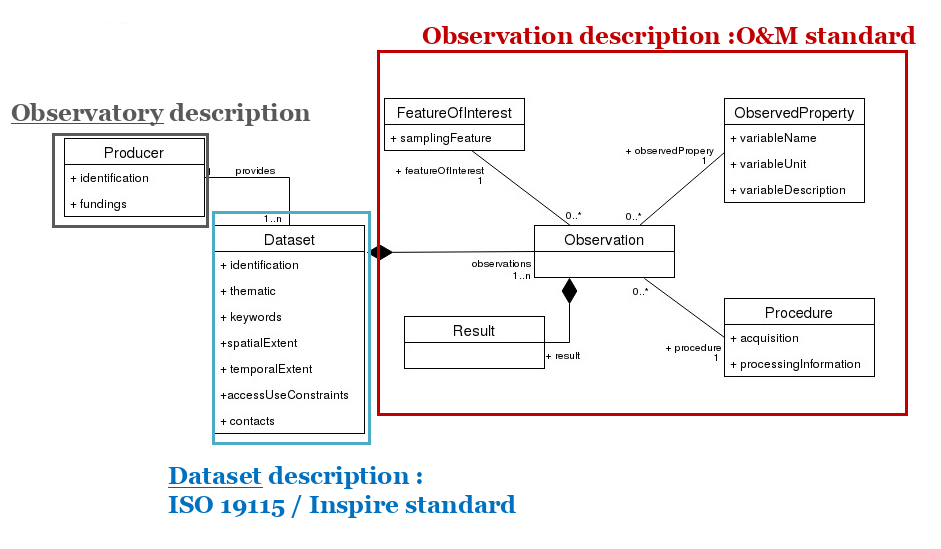
\includegraphics[width=\textwidth]{figures/theia_pivot_model.png}
	\caption{Figure from \url{https://github.com/theia-ozcar-is/csv-to-theia-ozcar-pivot-model}.}
\end{figure}


At the highest in the hierarchy are 3 JSON objects : 

\begin{itemize}
\item 	 producer;
\item 	 datasets;
\item 	 version.
\end{itemize}

datasets is a collection of dataset JSON object. Each dataset contains 3 informations : 

\begin{itemize}
\item 	 identifier;
\item 	 metadata;
\item 	 observations
\end{itemize}

observations is a collection of observation JSON object. producer, dataset and observation parameters are detailed in the sections below. 

% ==================================================================
\subsubsection{Producer metadata}

The producer metadata are : 

\begin{itemize}
\item 	 Identifier (M) : identifier for the observtories concerned by the Theia$\vert$OZCAR IS have already been provided to the concerned laboratories;
\item 	 Name (M) : name of the observatory;
\item 	 Title (M) : title of the data producer;
\item 	 Description (M) : a description of the data producer;
\item 	 Objective (R) : a summary of the scientific objectives of the data producer;
\item 	 Measured variables (R) : a summary of the variables observed by the data producer;
\item 	 Email (M) : generic email to contact the data producer;
\item 	 Contacts (M) : first names, last names, emails and roles of the data producer. 2 roles exist: Project leader and Data manager. The project leader is the scientific manager of the observatory, the Data manager is the person in charge of the data management;
\item 	 Funders (M) : types of organisations, scanR identifiers and names of the organisations that fund the data producer;
\item 	 Online resource (O) : link towards the website of the data producer, links to download data, doi and webservice. For the moment, the webservice type is not working.
\end{itemize}

% ==================================================================
\subsubsection{Dataset metadata}

The dataset metadata are : 

\begin{itemize}
\item 	 Identifier (M) : each dataset identifier is based on the data producer identifier as following : $PRODUCERID\_DAT\_DATASETID$;
\item 	 Title (M) : title of the dataset;
\item 	 Description (M) : summary of the dataset, such as definition of the measured variables, the purpose of the study or the geographic location;
\item 	 Subject (M) : lists of keywords and INSPIRE theme;
\item 	 Creator (M) : lists of contacts for the dataset (people in charge of the dataset). Same informations registered as in producer.contacts. 2 roles exist : Publisher and Principal investigator. A Publisher is the person in charge of the data management, the Principal investigator is the scientific referent of the dataset. At least one Principal investigator is required;
\item 	 Spatial coverage (M) : wkt object referencing the spatial extent of the dataset in latitude/longitude;
\item 	 Lineage (M) : describes the life cycle of the dataset, from the acquisition to the data entry via the data treatment.
\end{itemize}

% ==================================================================
\subsubsection{Observation metadata}

The observation metadata are : 

\begin{itemize}
\item 	 Identifier (M) : each dataset identifier is based on the data producer identifier as following : $PRODUCERID\_OBS\_DATASETID$;
\item 	 Processing level (O) : Raw data, Quality-controlled data, Derived products;
\item 	 Data type (M) : Numeric, Text, Vector, Raster, Photo, Video, Audio, Other;
\item 	 Temporal extent (M) : startDate/endDate, format ISO 8601 "YYYY-MM-DDThh:mm:ssZ";
\item 	 Observed property (M) : name of the variable of the observed phenomenon;
\item 	 Station name (M) : name of the acquisition station;
\item 	 Dataset (M) : identifier of the dataset whom the observation belongs to;
\item 	 Data file name (M) : name of the file containing the observations (.csv, .txt, .dat, etc.).
\end{itemize}

% ==================================================================
\subsection{Filling the metadata file}

First of all, one has to make sure (only user with administrator right) WEBOBS.rc is rightly configurated like it is shown below, in order to display anything Theia|OZCAR related and to make sure the file theia.rc will be filled. This last configuration file is important because it gathers the metadata the users want to send to Theia|OZCAR data portal.

\begin{figure}[!h]
	\centering
	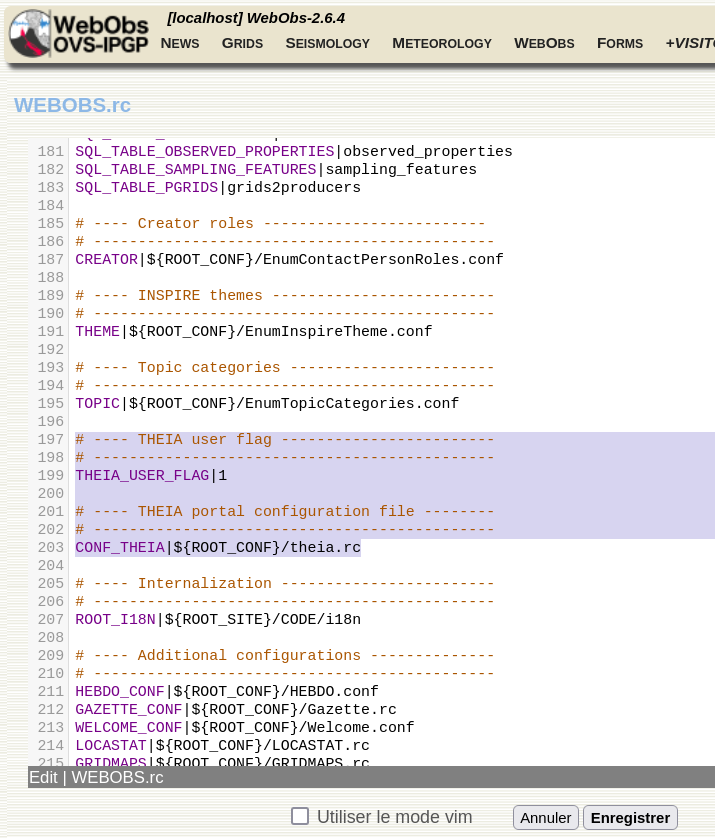
\includegraphics[width=\textwidth]{figures/webobs.rc.png}
	\caption{THIEA_USER_FLAG must be 1 to display the metadata resume board and anything metadata related.}
\end{figure}

Each of these 3 objects (producer, datasets, observations) can be filled through WebObs, and some are even done automatically, for example when creating a \wo{node}, or when filling a line of a calibration file. A table to display the producer, datasets and observations metadata is available. To do so, an user with administrator right has to create a link towards the showTHEIA.pl script through +ADMIN -> Admin editors -> MAIN MENU EDIT. 

\begin{figure}[!h]
	\centering
	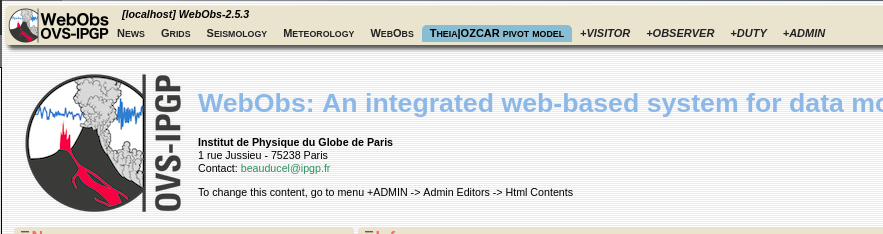
\includegraphics[width=\textwidth]{figures/theia_tab.png}
	\caption{Click on the tab to open the metadata summary table.}
\end{figure}

\begin{figure}[!h]
	\centering
	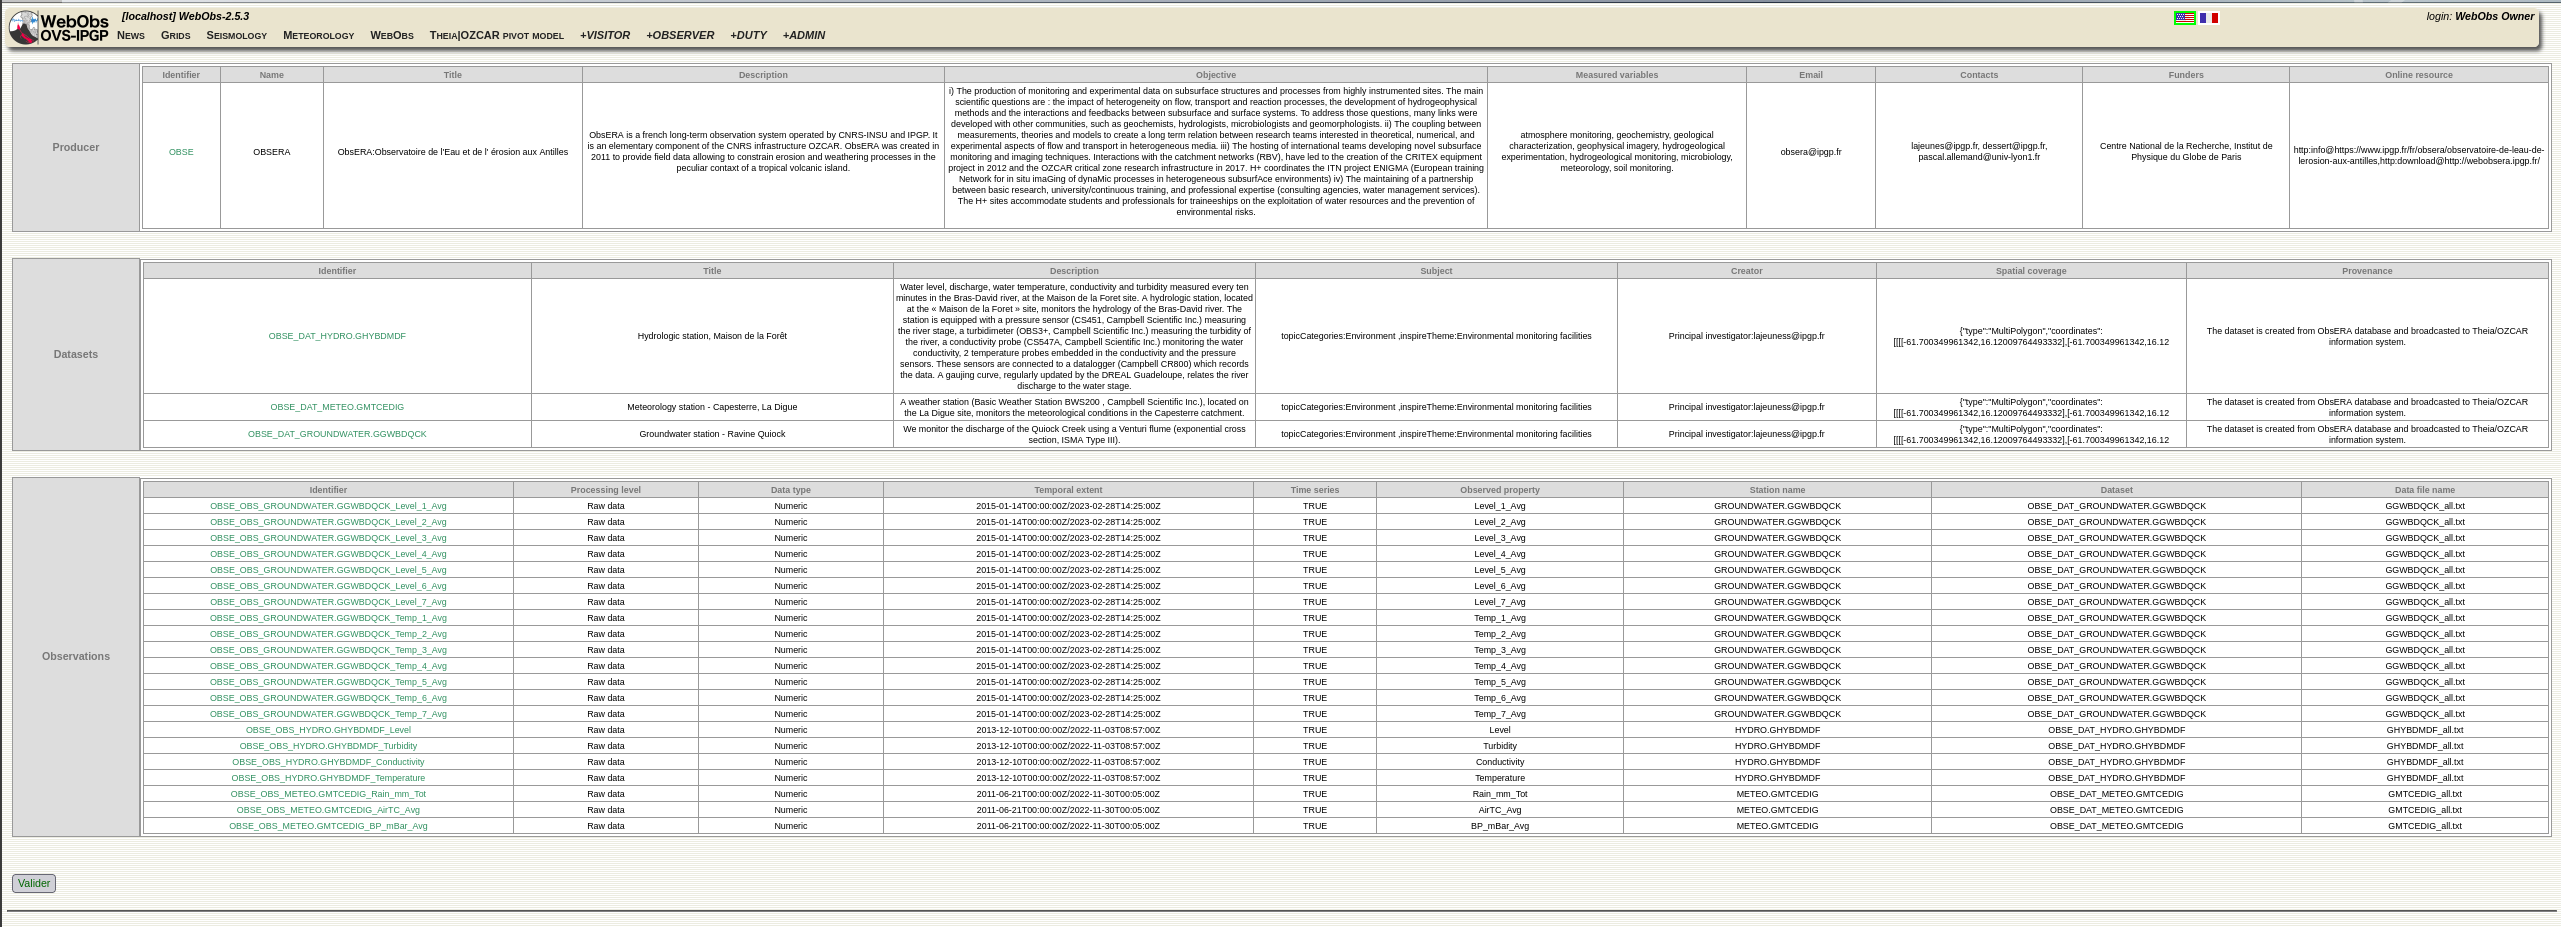
\includegraphics[width=\textwidth]{figures/theia_recap_table.png}
	\caption{The table sums up the mandatory metadata that have been filled to create the JSON file that will be send to the Theia$\vert$OZCAR IS.}
\end{figure}

By clicking on each row on the pencil, you can get back to the edition menu of the clicked object. If you click on the delete symbol, the row wil be deleted from the resume board but not from the database (which will happens when deleting a NODE or a variable in a given .clb file). Thus, only the rows displayed on the resume board will be integrated in the JSON file. Then, to validate the data you want to send in the JSON file, you have to validate the form. If all the required metadata are  validated, a message will appear to confirm the edition of the file called *theia.rc*. When launching the job, a .zip file is created for each dataset, containing the observations in a .txt file. Finally, a .zip file is made with the JSON and the datasets .zip files by creating a job using *sendTHEIA.pl* script (as shown below).

\newpage

\begin{figure}[!h]
	\centering
	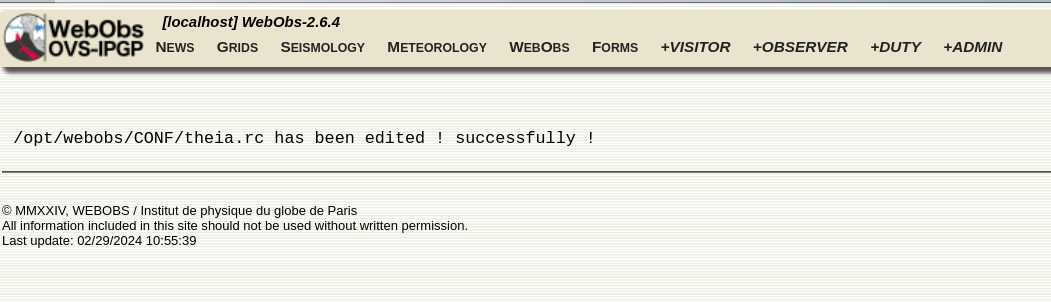
\includegraphics[scale=0.25]{figures/theia_rc.png}
	\caption{If it succeed, a configuration file containing all the information will be edited.}
\end{figure}

\begin{figure}[!h]
	\centering
	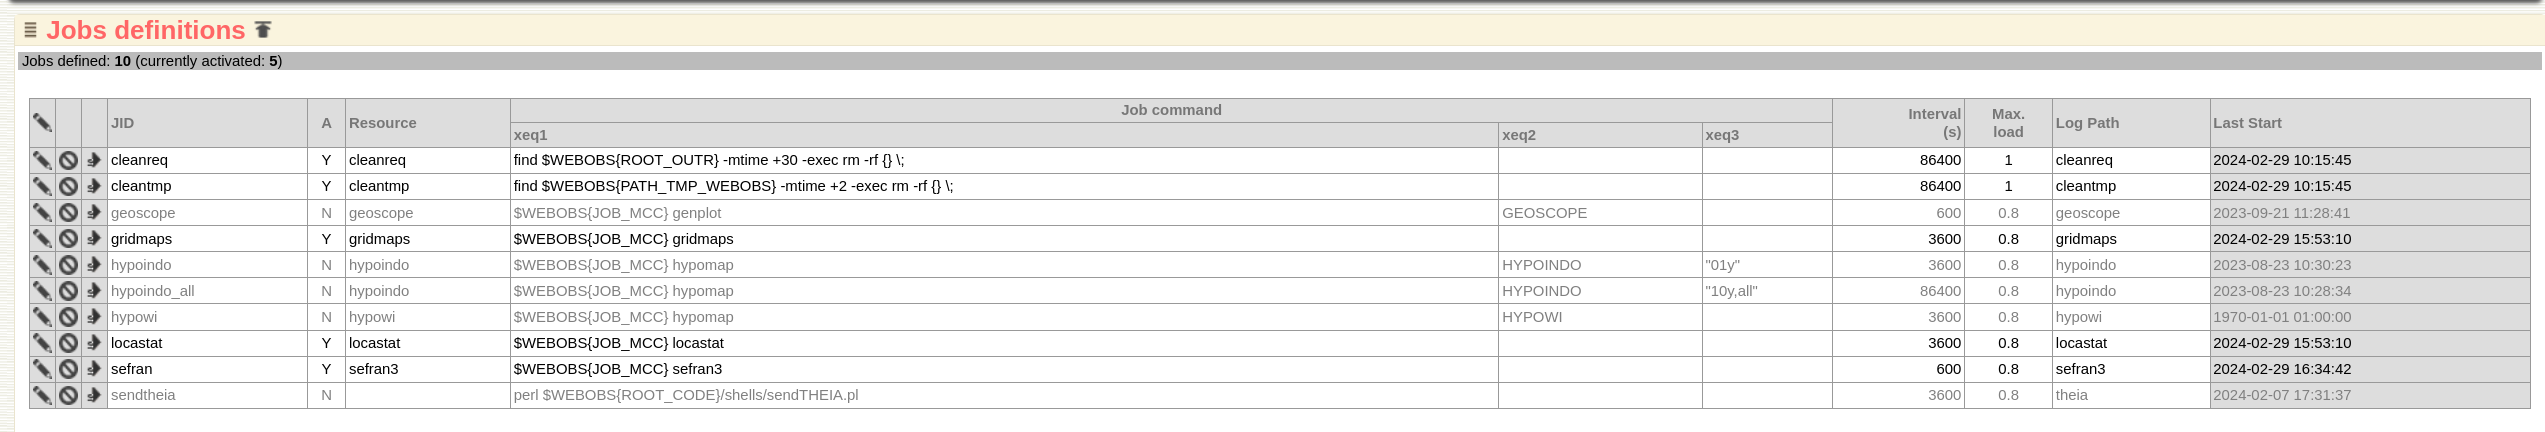
\includegraphics[scale=0.25]{figures/sendTHEIA.png}
	\caption{If it succeed, a .zip file will be downloaded in the OUTE/theia/ directory, containing all the metadata and data ready to send to THEIA pivot model.}
\end{figure}

\newpage

% ==================================================================
\subsubsection{Producer metadata}

The producer metadata can be filled throughout the \wo{domain} edition menu. 

\begin{figure}[!h]
	\centering
	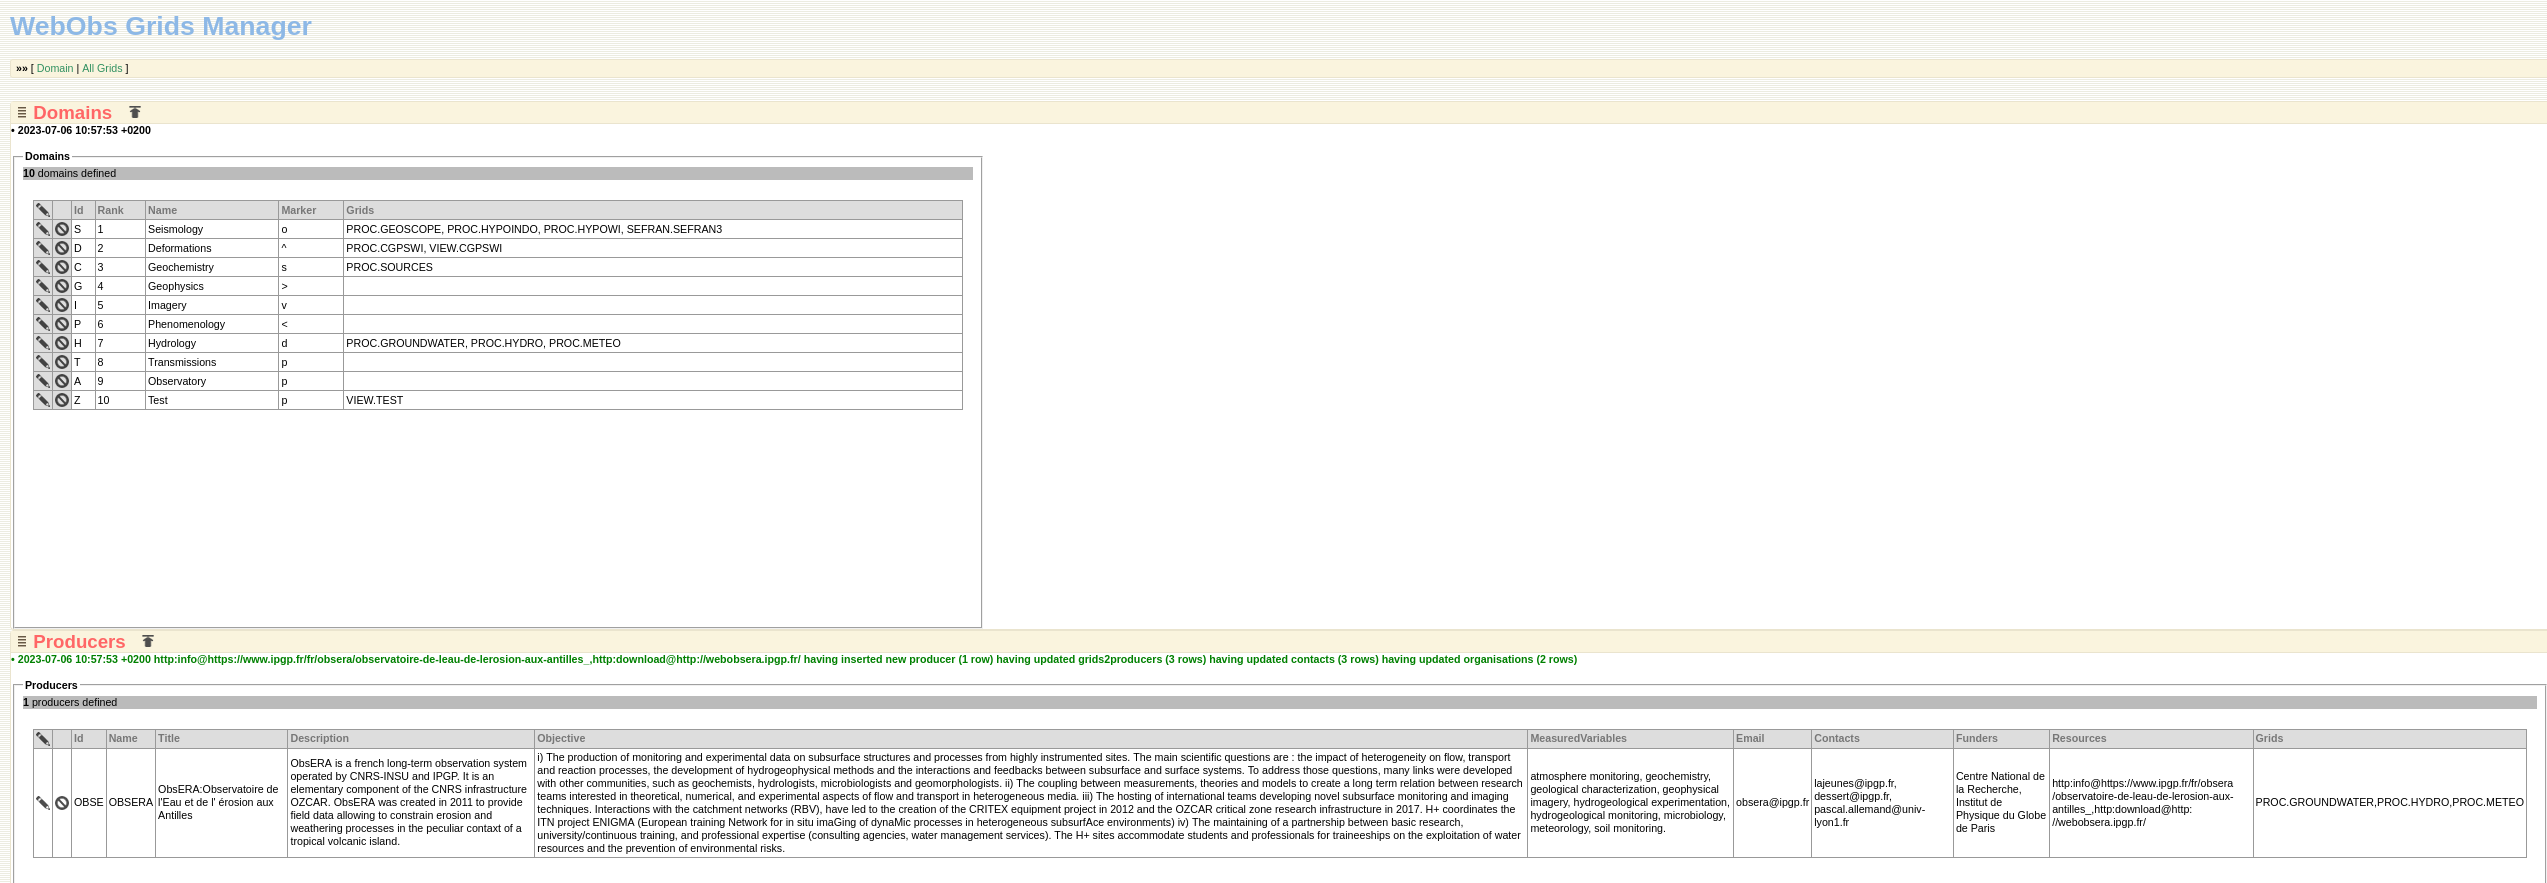
\includegraphics[width=\textwidth]{figures/gridsMgr.png}
	\caption{The table sums up the information about the data producer.}
\end{figure}

Each data producer can be edited or deleted. When creating, deleting or editing a producer, a local SQLite database is filled,  called WEBOBSMETA.db, which is only available for the admin. Only the mandatory metadata are necessary, in addition to the grids related to the producer (as several producer can co-exist on the same WebObs).Other metadata are optional even if some are more or less recommended.

\newpage

% ==================================================================
\subsubsection{Dataset metadata}

Dataset metadata is entered when creating or editing an existing \wo{node}. The \textbf{Name} WebObs \wo{node} fields correspond to the \textbf{dataset.Title} Theia$\vert$OZCAR IS field.

\begin{figure}[!h]
	\centering
	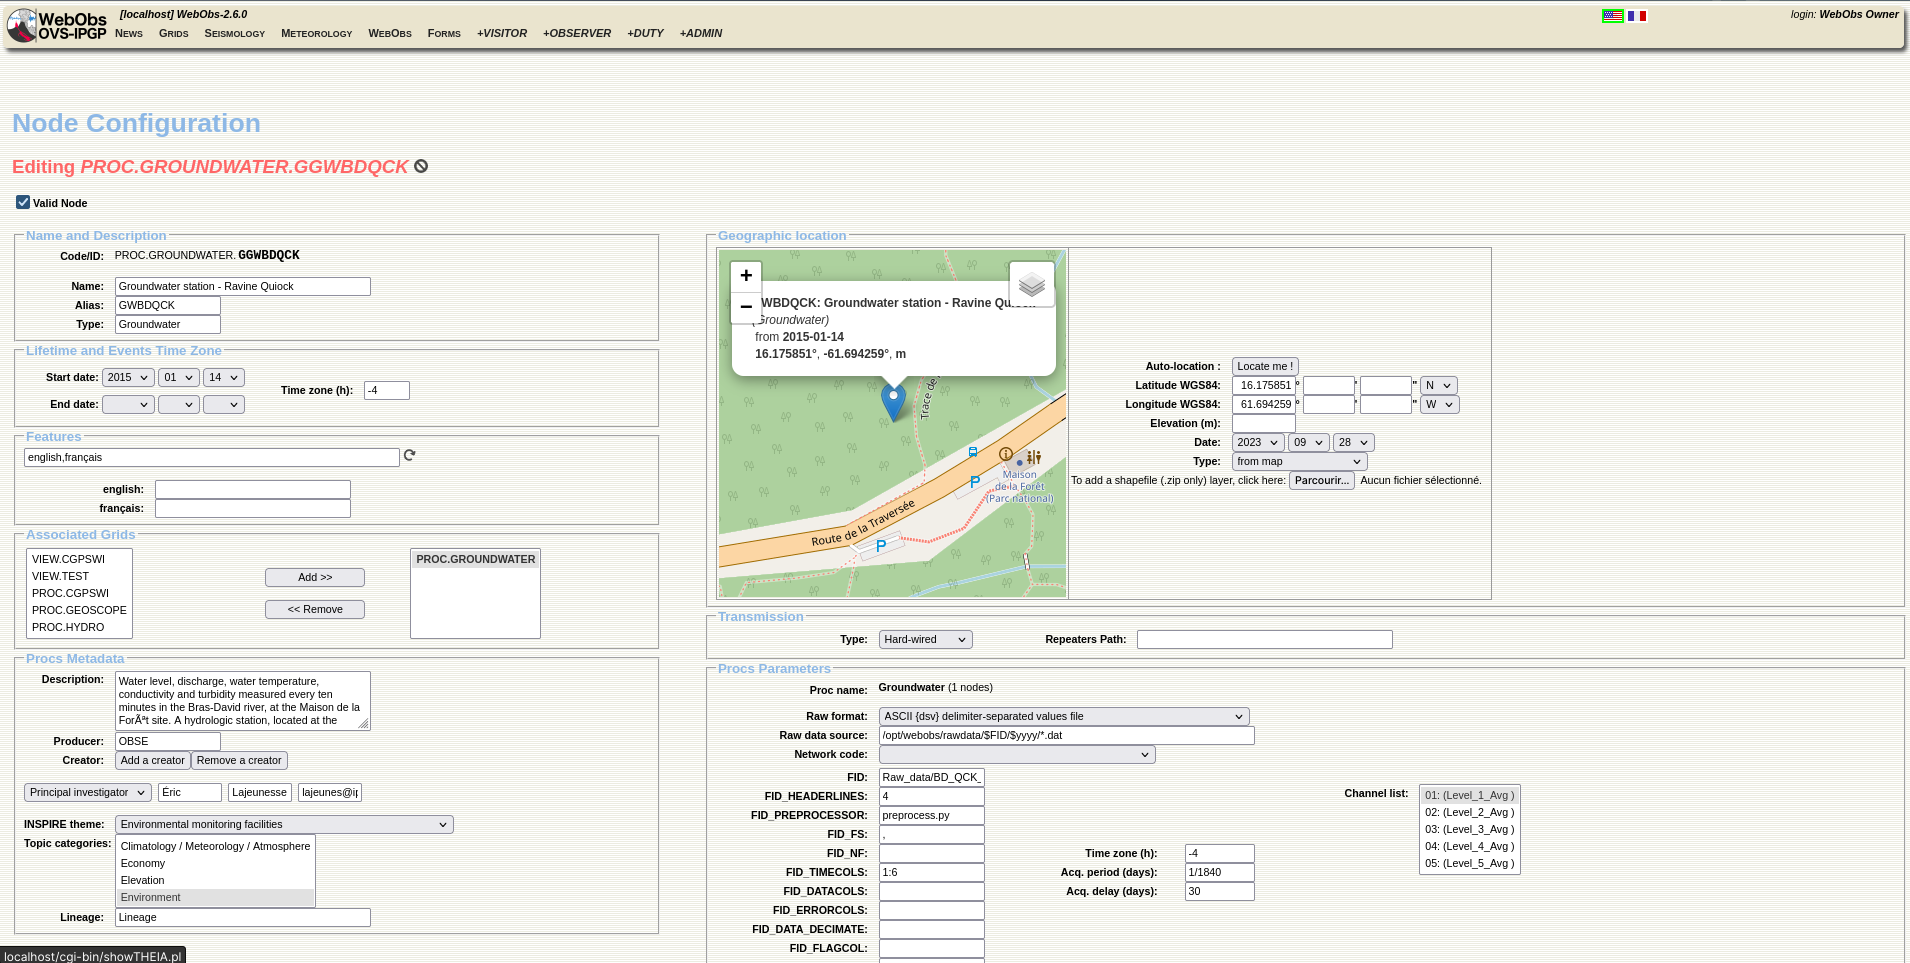
\includegraphics[width=\textwidth, scale=0.4]{figures/formNODE.png}
	\caption{When creating or editing a NODE, fields appear in the left lower panel to fill required metadata in.}
\end{figure}


% ==================================================================
\subsubsection{Observation metadata}

Observation metadata is entered when creating or editing an existing calibration file. Concerning the Theia topic categories, an hyperlink is provided towards the Theia$\vert$OZCAR Skosmos thesaurus.

\begin{figure}[!h]
	\centering
	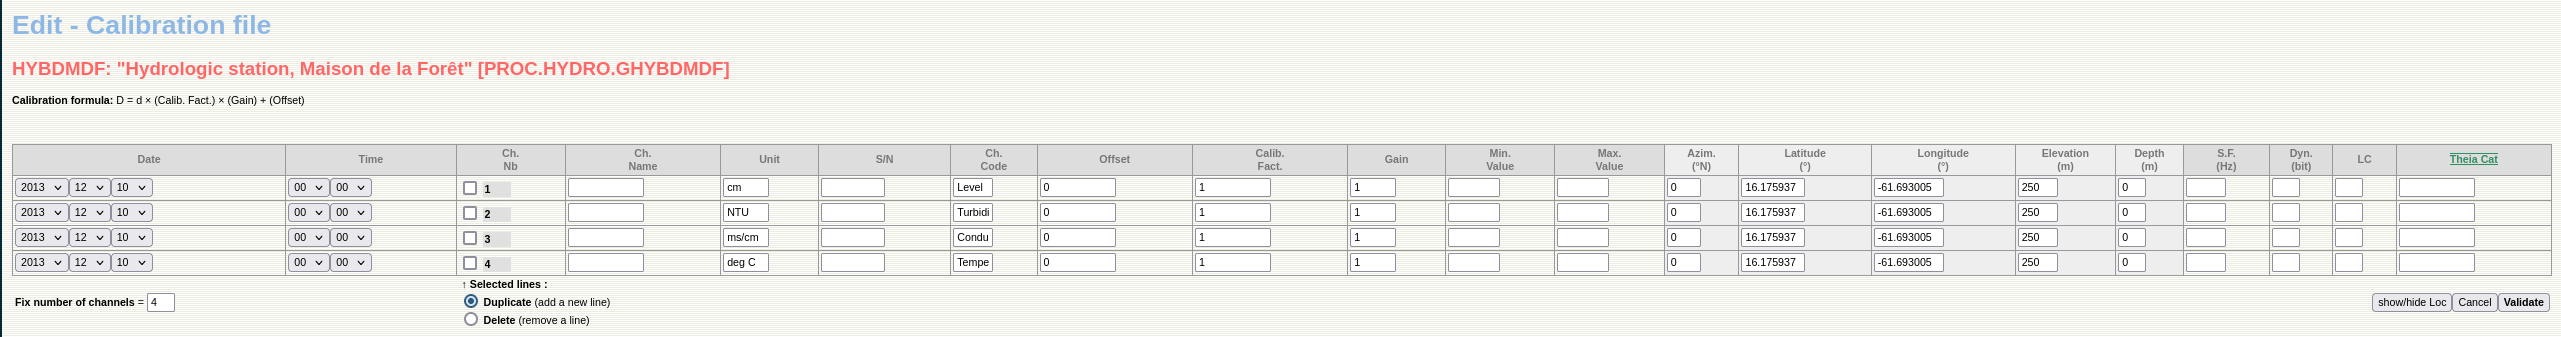
\includegraphics[width=\textwidth]{figures/calib_file_form.png}
	\caption{You can click on the highlighted Theia word (on the top right) to get driven to the Theia thesaurus.}
\end{figure}



%%%%%%%%%%%%%%%%%%%%%%%%%%%%%%%%%%%%%%%%%%%%%%%%%%%%%%%%%%%%%%%%%%%%
%%%%%%%%%%%%%%%%%%%%%%%%%%%%%%%%%%%%%%%%%%%%%%%%%%%%%%%%%%%%%%%%%%%%
\chapter{GENFORM tool} \label{metadata}



% ==================================================================
\section{What is GENFORM ?} \label{genform}

GENFORM is a WebObs integrated tool that allows to create \wo{form}. GENFORM can generates new \wo{form} by reading a configuration file (based on the key|value model) with a special syntax. Each \wo{form} is then associated to a table in a database called WEBOBSFORMS.db. Each table of the database contains data based on the following scheme :

\begin{center}
	\begin{tabular}{c c c}
		\hline
		\textit{Name} & \textit{Type} & \textit{Commentaire} \\
		\hline
		id & name & unique \\
		trash & boolean & True = bin	\\
		node & text & ID WebObs of the associated \wo{node} \\
		edate & datetime & date and time end of measurement/collection/sampling \\
		edate\_min & datetime & uncertainty date and time end of measurement \\
		sdate1 & datetime & date and time start of measurement/collection/sampling \\
		sdate1\_min & datetime & uncertainty date and time end of measurement \\
		users & text & WebObs ID of the operator (authorized list) \\
		input01 & text & data n°1 \\
		input02 & text & data n°2 \\
		... & text & data n°... \\
		comment & text \\
		tsupd & timestamp & last edit timestamp \\
		userupd & text & last edit user ID \\
		\hline
	\end{tabular}
\end{center}

Once a \wo{form} is created through GENFORM, the given \wo{form} works like a normal \wo{form} in WebObs.

\section{Creation of a FORM} \label{genform_creation}

To create a new \wo{form} using GENFORM, you have to go in the \wo{grid} menu list and click on the pencil next to \textbf{Raw Data}. Then, you have to chose a name for the FORM and select a template that will be used to help you through the creation process. Currently, 3 templates exist : 

\begin{itemize}
	\item GENFORM: the most basic template that shows you all the different types of inputs that you can use in GENFORM
	\item EAUX: a template based on the old EAUX \wo{form} used for the water chemistry
	\item GAZ: a template based on the old GAZ \wo{form} used for the gas chemistry
\end{itemize}

\begin{figure}[!h]
	\centering
	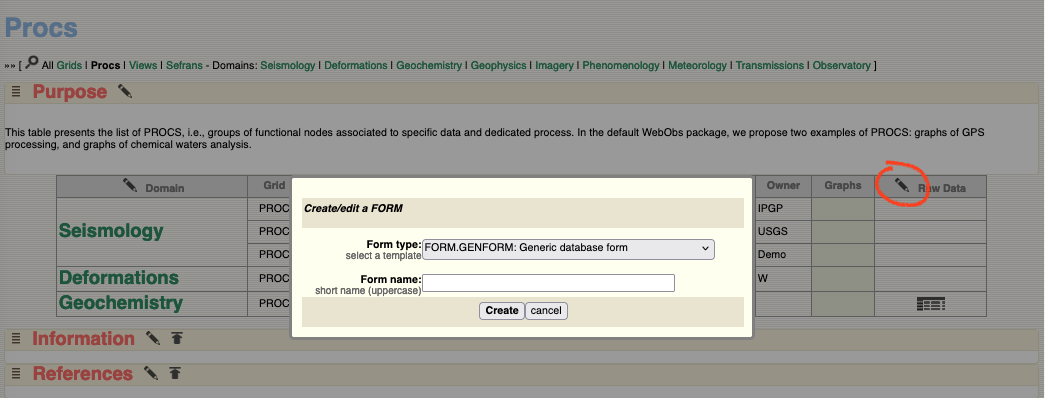
\includegraphics[width=\textwidth]{figures/GENFORM_creation.png}
	\caption{Chose a name and a template and click on Create.}
	\label{GENFORM_creation}
\end{figure}

If you want to edit a \wo{form}, you just need to go in the GENFORM creation menu and write the name of the \wo{form} you want to edit, no matter the template which is selected.

\section{The GENFORM language}

Each GENFORM is formed of COLUMNS. Each COLUMN contains FIELDSETS. Each FIELDSET contains INPUTS. An INPUT has a NAME, a UNIT and a TYPE. 3 TYPES exist for the moment:

\begin{itemize}
	\item formula, which allows to make simple mathematical operations between the different INPUTS
	\item list, which allows to use a configuration file to create select input in the form
	\item text (work in progress)
\end{itemize}

Each FIELDSET has a NAME, a number of COLUMNS and the NAME of the INPUTS you to display in each COLUMN. Each COLUMN has a list of the FIELDSETS you want to display in each COLUMN.

Finally, the configuration file of the \wo{form} has a NAME, that you have chosen at the creation of the \wo{form}, a BANG, which is the begininng year of the dataset associated to the \wo{form}, a title, to display in the \wo{grid} form, column and fieldset numbers and a STARTING\_DATE key which is a boolean that allows GENFORM to display or not display a starting date when filling a record form.



% ==================================================================
\backmatter

%%%%%%%%%%%%%%%%%%%%%%%%%%%%%%%%%%%%%%%%%%%%%%%%%%%%%%%%%%%%%%%%%%%%
%%%%%%%%%%%%%%%%%%%%%%%%%%%%%%%%%%%%%%%%%%%%%%%%%%%%%%%%%%%%%%%%%%%%

\chapter{Appendix}

% ==================================================================

\begin{table}[htp]
\caption{Data raw formats for PROCS}
\label{rawformats}
\lstinputlisting{../../CODE/etc/rawformats.conf}
\end{table}


% ==================================================================
\begin{table}[htp]
\caption{Time scale keys (\textit{x} is an integer).}
\label{timescales}
\begin{center}
\begin{tabular}{|c|l|}
\hline
\textbf{Key} & \textbf{Time scale}\\
\hline
x\texttt{s}  & x seconds\\
x\texttt{n}  & x minutes\\
x\texttt{h}  & x hours\\
x\texttt{d}  & x days\\
x\texttt{w}  & x weeks\\
x\texttt{m}  & x months\\
x\texttt{y}  & x years\\
x\texttt{l}  & last x data\\
\texttt{r}x  & reference to date \wokey{REFx\_DATE}\\
\texttt{all}  & all data\\
\hline
\end{tabular}
\end{center}
\end{table}

% ==================================================================
\begin{table}[htp]
\caption{Marker type list}
\label{markertype}
\begin{center}
\begin{tabular}{|c|l|}
\hline
\textbf{Symbol} & \textbf{Marker}\\
\hline
\texttt{.}  & Point\\
\texttt{+}  & Plus sign\\
\texttt{*}  & Asterisk\\
\texttt{x}  & Cross\\
\texttt{o}  & Circle\\
\texttt{s}  & Square\\
\texttt{d}  & Diamond (vertical rhombus)\\
\texttt{\textasciicircum} & Upward-pointing triangle\\
\texttt{v}  & Downward-pointing triangle\\
\texttt{\textgreater} & Right-pointing triangle\\
\texttt{\textless} & Left-pointing triangle\\
\texttt{p}  & Five-pointed star (pentagram)\\
\texttt{h}  & Six-pointed star (hexagram)\\
\hline
\end{tabular}
\end{center}
\end{table}


% ==================================================================
\begin{table}[htp]
\caption{Line Style list}
\label{linestyle}
\begin{center}
\begin{tabular}{|c|l|}
\hline
\textbf{Symbol} & \textbf{Line style}\\
\hline
\texttt{-}  & Solid line\\
\texttt{--}  & Dashed line\\
\texttt{:}  & Dotted line\\
\texttt{-.}  & Dash-dot line\\
\hline
\end{tabular}
\end{center}
\end{table}


% ==================================================================
\begin{table}[htp]
\caption{Some basic R,G,B colors}
\label{rgbcolors}
\begin{center}
\begin{tabular}{|c|l|}
\hline
\textbf{R,G,B} & \textbf{Color}\\
\hline
\texttt{0,0,0}  & Black\\
\texttt{1,1,1}  & White\\
\texttt{1,0,0}  & Red\\
\texttt{0,1,0}  & Green\\
\texttt{0,0,1}  & Blue\\
\texttt{1,1,0}  & Yellow\\
\texttt{1,0,1}  & Magenta\\
\texttt{0,1,1}  & Cyan\\
\hline
\end{tabular}
\end{center}
\end{table}


% ==================================================================
% note: thumbnails colormaps are made with:
%       >> imwrite(shiftdim(repmat(jet(100),1,1,10),2),'jet.png')

\begin{table}[htp]
\caption{Some built-in colormaps}
\label{colormaps}
\begin{center}
\setlength{\fboxsep}{1pt}
\begin{tabular}{|c|l|}
\hline
\textbf{Name} & \textbf{Description}\\
\hline
\texttt{ryb}  & \fbox{
\includegraphics[width=3cm]{figures/ryb.png}}\\
\texttt{spectral}  & \fbox{
\includegraphics[width=3cm]{figures/spectral.png}}\\
\texttt{roma}  & \fbox{
\includegraphics[width=3cm]{figures/roma.png}}\\
\texttt{vik}  & \fbox{
\includegraphics[width=3cm]{figures/vik.png}}\\
\texttt{landcolor}  & \fbox{\includegraphics[width=3cm]{figures/landcolor.png}}\\
\texttt{seacolor}  & \fbox{\includegraphics[width=3cm]{figures/seacolor.png}}\\
\texttt{white}  & \fbox{\includegraphics[width=3cm]{figures/white.png}}\\
\texttt{gray}  & \fbox{\includegraphics[width=3cm]{figures/gray.png}}\\
\texttt{hot}  & \fbox{\includegraphics[width=3cm]{figures/hot.png}}\\
\texttt{jet}  & \fbox{\includegraphics[width=3cm]{figures/jet.png}}\\
\texttt{hsv}  & \fbox{\includegraphics[width=3cm]{figures/hsv.png}}\\
\texttt{cool}  & \fbox{\includegraphics[width=3cm]{figures/cool.png}}\\
\texttt{bone}  & \fbox{\includegraphics[width=3cm]{figures/bone.png}}\\
\texttt{pink}  & \fbox{\includegraphics[width=3cm]{figures/pink.png}}\\
\texttt{copper}  & \fbox{\includegraphics[width=3cm]{figures/copper.png}}\\
\texttt{spring}  & \fbox{\includegraphics[width=3cm]{figures/spring.png}}\\
\texttt{summer}  & \fbox{\includegraphics[width=3cm]{figures/summer.png}}\\
\texttt{autumn}  & \fbox{\includegraphics[width=3cm]{figures/autumn.png}}\\
\texttt{winter}  & \fbox{\includegraphics[width=3cm]{figures/winter.png}}\\
\hline
\end{tabular}
\end{center}
\end{table}


% ==================================================================
\begin{table}[htp]
\caption{Date string format list. ``Datenum'' column indicates if the format is valid for date/time string as key value}
\label{datestr}
\begin{center}
\begin{tabular}{|c|c|l|l|l|}
\hline
\textbf{Number} & \textbf{Datenum} & \textbf{String} & \textbf{Example} & \textbf{Comment}\\
\hline
\texttt{-1}		&		& automatic					&	& default value\\
\texttt{0}		& OK	& 'dd-mmm-yyyy HH:MM:SS'	& 01-Mar-2000 15:45:17	&\\
\texttt{1}		& OK	& 'dd-mmm-yyyy'				& 01-Mar-2000	&\\
\texttt{2}		&		& 'mm/dd/yy'				& 03/01/00	&\\
\texttt{3}		&		& 'mmm'						& Mar	&\\
\texttt{4}		&		& 'm'						& M	&\\
\texttt{5}		&		& 'mm'						& 03	&\\
\texttt{6}		&		& 'mm/dd'					& 03/01	&\\
\texttt{7}		&		& 'dd'						& 01	&\\
\texttt{8}		&		& 'ddd'						& Wed	&\\
\texttt{9}		&		& 'd'						& W	&\\
\texttt{10}		&		& 'yyyy'					& 2000	&\\
\texttt{11}		&		& 'yy'						& 00	&\\
\texttt{12}		&		& 'mmmyy'					& Mar00	&\\
\texttt{13}		&		& 'HH:MM:SS'				& 15:45:17	&\\
\texttt{14}		&		& 'HH:MM:SS PM'				& 3:45:17 PM	&\\
\texttt{15}		&		& 'HH:MM'					& 15:45	&\\
\texttt{16}		&		& 'HH:MM PM'				& 3:45 PM	&\\
\texttt{17}		&		& 'QQ-YY'					& Q1-96	&\\
\texttt{18}		&		& 'QQ'						& Q1	&\\
\texttt{19}		&		& 'dd/mm'					& 01/03	&\\
\texttt{20}		&		& 'dd/mm/yy'				& 01/03/00	&\\
\texttt{21}		&		& 'mmm.dd,yyyy HH:MM:SS'	& Mar.01,2000 15:45:17	&\\
\texttt{22}		&		& 'mmm.dd,yyyy'				& Mar.01,2000	&\\
\texttt{23}		& OK	& 'mm/dd/yyyy'				& 03/01/2000	&\\
\texttt{24}		&		& 'dd/mm/yyyy'				& 01/03/2000	&\\
\texttt{25}		&		& 'yy/mm/dd'				& 00/03/01	&\\
\texttt{26}		&		& 'yyyy/mm/dd'				& 2000/03/01	&\\
\texttt{27}		&		& 'QQ-YYYY'					& Q1-1996	&\\
\texttt{28}		&		& 'mmmyyyy'					& Mar2000	&\\
\texttt{29}		& OK	& 'yyyy-mm-dd'				& 2000-03-01	& ISO 8601\\
\texttt{30}		& OK	& 'yyyymmddTHHMMSS'			& 20000301T154517	& ISO 8601\\
\texttt{31}		& OK	& 'yyyy-mm-dd HH:MM:SS'		& 2000-03-01 15:45:17	&\\
\hline
\end{tabular}
\end{center}
\end{table}


% ==================================================================
\begin{table}[htp]
\caption{TeX stream modifiers and main escape characters allowed in titles and labels when specified, in addition to standard Greek letters and mathematical symbols.}
\label{texcommands}
\begin{center}
\begin{tabular}{|c|l|}
\hline
\textbf{TeX Modifier} & \textbf{Comment}\\
\hline
\texttt{\^}  & Superscript or exponent (use braces for more than 1 character)\\
\texttt{\_}  & Subscript (use braces for more than 1 character)\\
\texttt{$\backslash$bf}  & Bold font\\
\texttt{$\backslash$it}  & Italic font\\
\texttt{$\backslash$rm}  & Normal font\\
\texttt{$\backslash$fontname\{fontname\}}  & Specify the name of the font family to use\\
\texttt{$\backslash$fontsize\{fontsize\}}  & Specify the font size in FontUnits\\
\texttt{$\backslash$color(colorSpec)}  & Specify color for succeeding characters\\
\hline
\texttt{$\backslash$backslash}  & backslash character\\
\texttt{$\backslash$\{} or \texttt{$\backslash$lbrace}  & left brace character\\
\texttt{$\backslash$\}} or \texttt{$\backslash$rbrace}  & right brace character\\
\texttt{$\backslash$\_}  & underscore (low line) character\\
\texttt{$\backslash$\^} or \texttt{$\backslash$hat}  & hat character\\
\hline
\end{tabular}
\end{center}
\end{table}

% ==================================================================

\begin{table}
\caption{Suggestion for NODE ID code: \texttt{\textbf{N D T S S S S}}}
\label{nodeidcodes}
\begin{center}
\begin{tabular}{|c|c|l|}
\hline
\textbf{Letter} & \textbf{Code} & \textbf{Comment}\\
\hline
\texttt{N} = Network         & \texttt{I}	&	IPGP\\
      			             & \texttt{G}	&	OVSG\\
      			             & \texttt{M}	&	OVSM\\
      			             & \texttt{R}	&	OVPF\\
      			             & \texttt{P}	&	PVMBG\\
\hline
\texttt{D} = Domain          & \texttt{S}	&	Seismology\\
      			             & \texttt{D}	&	Deformations\\
      			             & \texttt{G}	&	Geophysics\\
      			             & \texttt{C}	&	Chemistry\\
      			             & \texttt{I}	&	Imagery\\
      			             & \texttt{M}	&	Meteorology\\
      			             & \texttt{P}	&	Phenomenology\\
      			             & \texttt{A}	&	Acquisition\\
\hline
\texttt{DT} = Technique      & \texttt{SB}	&	Broad-band\\
      			             & \texttt{SZ}	&	Short-period\\
      			             & \texttt{SA}	&	Acceleration\\
      			             & \texttt{ST}	&	Temporary\\
      			             & \texttt{DC}	&	Continuous GNSS\\
      			             & \texttt{DT}	&	Tilmetry\\
      			             & \texttt{DD}	&	Distancemetry\\
      			             & \texttt{DE}	&	Extensometry\\
      			             & \texttt{GM}	&	Magnetometry\\
      			             & \texttt{GE}	&	Electric\\
      			             & \texttt{CS}	&	Hot Springs Analysis\\
      			             & \texttt{CG}	&	Gas Analysis\\
      			             & \texttt{CD}	&	DOAS\\
      			             & \texttt{IV}	&	Visible Imaging\\
      			             & \texttt{IT}	&	Thermal Imaging\\
      			             & \texttt{MW}	&	Weather station\\
      			             & \texttt{PJ}	&	Journal Phenomenology\\
      			             & \texttt{PE}	&	Eruption\\
      			             & \texttt{AI}	&	Infrastructures\\
      			             & \texttt{AT}	&	Transmission\\
      			             & \texttt{AB}	&	Buildings\\
\hline
\end{tabular}
\end{center}
\end{table}

% ==================================================================

\begin{table}
\caption{\wokey{*\_ARROWSHAPE} key's parameter syntax is a 4-element vector of scalars, coma or space separated = \wokey{HEADW,HEADL,HEADI,LINEW}. Values are ratios relative to the length of reference scale legend arrow equals 1 (see \wofile{CODE/matlab/arrows.m} for further details).}
\label{arrowshape}
\begin{center}
\begin{tabular}{|c|c|l|}
\hline
\textbf{Parameter} & \textbf{Default value} & \textbf{Comment}\\
\hline
\texttt{HEADW}	& 0.15	& arrow's head width\\
\hline
\texttt{HEADL}	& 0.15	& arrow's head length\\
\hline
\texttt{HEADI}	& 0.12	& arrow's head inside length\\
\hline
\texttt{LINEW}	& 0.03	& arrow's line width\\
\hline
\end{tabular}
\end{center}
\label{nodeidcodes}
\end{table}

%%%%%%%%%%%%%%%%%%%%%%%%%%%%%%%%%%%%%%%%%%%%%%%%%%%%%%%%%%%%%%%%%%%%
%%%%%%%%%%%%%%%%%%%%%%%%%%%%%%%%%%%%%%%%%%%%%%%%%%%%%%%%%%%%%%%%%%%%

\chapter{Acknowledgments}


A 15-year history summary.

\textbf{Episode I}. The \webobs project was born in September 2000 when \textit{François Beauducel} has been assigned to the Guadeloupe volcanological observatory in Lesser Antilles. First ideas of an integrated monitoring and management system have risen thanks to fruitful discussions with \textit{Christian Anténor-Habazac}, \textit{Jean-Christophe Komorowski} and \textit{Stéphane Acounis}. Quickly (and dirtily) developed in about a year of sparse hours, a first version of \webobs was presented in Paris on January 2002 \citep{beauducel2002qes}, containing most of the present content: station files, networks, automatic graphs for seismic, deformation, geochimia and weather stations, shared calendar... During the first two years of the project, there was a single developer, moreover, a scientist during its overtime work and not a dedicated computer specialist!

\textbf{Episode II}. From August 2002 to December 2005, \textit{Didier Mallarino} was the first computer engineer who invested a part of its time to improve the codes and configuration files, especially by developing more robust and flexible Perl GCI scripts \citep{beauducel2004webovs,beauducel2005wim,beauducel2006sov}. In 2004, a version of \webobs has been partially duplicated and adapted for a public website (CDSA).

\textbf{Episode III}. From 2006 to 2010, some code improvements where made by a second computer engineer \textit{Alexis Bosson}: particularly, the system was internationalized and a first effort was made to integrate \webobs with observatory acquisition chain seismology standards \citep{beauducel2010webobs}. During these years, the system worked in a relatively stable production state, and it was adapted and partly installed in different observatories: Paris (thanks to \textit{François Truong} \citep{truong2009magis}), Addis-Abeba (thanks to \textit{Alexandre Nercessian}), Martinique (thanks to \textit{Jean-Marie Saurel} and \textit{Benoît Costes}), Montserrat (thanks to \textit{Alexis Bosson} and \textit{Roderick Stewart}) and later in 2012 at La Réunion (thanks to \textit{Patrice Boissier} and \textit{Philippe Kowalski}).

\textbf{Episode IV} (\textit{A New Hope}). In 2012, \webobs obtained its first dedicated funding support from the French Ministry of Ecology, thanks to \textit{Steve Tait}, \textit{Arnaud Lemarchand} and \textit{Pierre Agrinier}. A very significant contribution has been made by \textit{Didier Lafon}, the first computer engineer working 100\% on the project. Taking advantage of 10 years of production feedback, he reassessed the whole coding concept, improved and standardized the codes, made library modules and administration tools, wrote technical documentation, put all this under a versioning control system and built the first Linux installation package. This allowed to install a first alpha and beta version at Merapi observatory (thanks to \textit{Ali A. Fahmi}), then the same codes in Guadeloupe, Martinique and La Réunion observatories, and start a real collaborative development. During this last period, we welcomed additional contributors, as developers or end-users: \textit{Xavier Béguin}, \textit{Jean-Marie Saurel}, \textit{Stephen Roselia}, \textit{Patrice Boissier}, \textit{Laura Henriette}, and of course all the observatory teams under the direction and enthousiast support of \textit{Jean-Bernard de Chabalier}, \textit{Valérie Clouard}, \textit{Andrea Di Muro}, \textit{Nicolas Villeneuve}, \textit{Céline Dessert}, \textit{Aline Peltier}, \textit{Roberto Moretti}, and \textit{Anne-Marie Lejeune}.

\textbf{Episode V}. In October 2018, \webobs code has been released on \url{https://github.com/IPGP/webobs}.
\bibliographystyle{plain}
\bibliography{references}


\end{document}
\end
